%\documentclass[fleqn,reqno,a4paper,parskip=half]{scrartcl}
\documentclass[fleqn,reqno,a4paper,parskip=half]{scrbook}
%\usepackage{showkeys}      % zeigt label-Bezeichner an

%%%%%%%%%%%%%%%%   Pakete   %%%%%%%%%%%%%%%%%%

\usepackage{charter} %Charter fuer englische Texte
%\linespread{1.05} % Durchschuss für Charter leicht erhöhen

%\usepackage[mathletters]{ucs} %direkt griechisches im Mathe modus
%\usepackage[utf8]{inputenc}
\usepackage[utf8]{inputenc}
%\usepackage[utf8x]{inputenc}
%\usepackage[T1]{fontenc}
%\usepackage{times}

% utf8x is incompatible with biblatex, the following trick is a remedy
% source: https://tex.stackexchange.com/a/213177
\input{binhex}
\makeatletter
\def\uc@dclc#1#2#3{%
  \ifnum\pdfstrcmp{#2}{mathletters}=\z@
    \begingroup\edef\x{\endgroup
      \noexpand\DeclareUnicodeCharacter{\hex{#1}}}\x{#3}%
  \fi
}
\input{uni-3.def}
\def\uc@dclc#1#2#3{%
  \ifnum\pdfstrcmp{#2}{default}=\z@
    \begingroup\edef\x{\endgroup
      \noexpand\DeclareUnicodeCharacter{\hex{#1}}}\x{#3}%
  \fi
}
\input{uni-34.def}
\makeatother






%TODO_Lorin: besser?
   %\usepackage{uniinput}       % für Unicode-Zeichen, wird momentan nicht verwendet, deshalb auskommentiert by Benni


%\usepackage[ngerman]{babel}
%\usepackage{ngerman}
\usepackage[tbtags,sumlimits,intlimits,namelimits]{amsmath}

\usepackage{amsfonts}
\usepackage{amssymb}
\usepackage{bbm}
\usepackage{ulem}
\usepackage{tikz}
\usepackage{pgf}
\usepackage{ifpdf}
\usepackage{color}
\usepackage{esint}
\usepackage{framed}
\usepackage{wasysym}  % \ocircle
%\usepackage{calc}   % \begin{tabular}[b]{|p{\textwidth-2\tabcolsep}|}

%\usepackage[colorlinks=true,linkcolor=black,citecolor=black,urlcolor=black]{hyperref}  % print
\usepackage[colorlinks=true,linkcolor=blue,citecolor=blue]{hyperref}    % web
\usepackage[top=2.3cm, bottom=3.45cm, left=2.3cm, right=2.3cm]{geometry}
%\numberwithin{equation}{section}
\usepackage{chngcntr}
\counterwithin*{section}{part}
%\graphicspath{{images/png/}{images/}}        % Pfad, in dem sich Grafikdateien befinden
%\usepackage{subfigure}          % Unterbilder, deprecated
%\usepackage(subfig}

\usepackage[all]{hypcap}
%\usepackage{cite}           % Literatur
\usepackage{graphicx}       % Bilder in Tabellen
\usepackage{float}          % eigene Float-Umgebungen, H-Option, um Bilder an der aktuellen Stelle anzuzeigen
\usepackage{caption}
\usepackage{subcaption,array}
%\usepackage{array}

\restylefloat{figure}       % Bilder an der Stelle, wo sie eingebunden werden
\usepackage{multirow}
\usepackage{listings}       % Darstellung von Source-Code
\usepackage{framed}         % Rahmen um Text
\usepackage{arydshln}       % gestrichelte Linie in Tabelle mit \hdashline
\usepackage{longtable}     % Tabellen mit automatischen Seitenumbruch
\usepackage{layouts}        % textwidth in cm: \printinunitsof{cm}\prntlen{\textwidth}
 % \cref verbessert
\usepackage[
  % capitalize names automatically
  capitalise,
  % mark all of "Lemma 1" as a link, not only "1"
  nameinlink,
  % pass language used in document to enable cleveref in otherlanguage env
  ngerman,english,
]{cleveref}
%\usepackage{ziffer}       % Komma in Dezimalzahlen
\usepackage{url}          % Links
%% end old
\definecolor{darkblue}{rgb}{0,0,.5}
\definecolor{black}{rgb}{0,0,0}

\usepackage[framemethod=TikZ]{mdframed}       % Rahmen um Text und Gleichungen


%\usepackage{arydshln}      % gestrichelte Linie in Tabelle mit \hdashline
\usepackage{dirtytalk}          % \say{...} erzeugt (deutsche) Anführungszeichen

\usepackage{tipa}
\usepackage{transparent}    % needed for inkscape generated pdf_tex files
\usepackage{multicol}       % multiple columns
\usepackage{moreverb}       % verbatimwrite
\usepackage{verbatimbox}    % \begin{verbbox}
\usepackage{booktabs}
\usepackage{morefloats}     % Increase the number of simultaneous LaTeX floats
\usepackage{enumitem}       % more control oover itemize
%\usepackage{algorithm2e}
%\usepackage{algorithmic}
%\usepackage{algpseudocode}

\newsavebox\lstbox
\mdfdefinestyle{MyFrame}{%
    innertopmargin=0pt,
    innerbottommargin=10pt,
    innerrightmargin=20pt,
    innerleftmargin=20pt}

\definecolor{darkgreen}{HTML}{009900}
    
% settings for algorithm
\lstset{literate=%
    {Ö}{{\"O}}1
    {Ä}{{\"A}}1
    {Ü}{{\"U}}1
    {ß}{{\ss}}1
    {ü}{{\"u}}1
    {ä}{{\"a}}1
    {ö}{{\"o}}1
    {⇐}{{$\leftarrow$}}1
    {>=}{{$\geq$}}1
    {~}{{\textasciitilde}}1,  
  language=C++,
  numbers=none,
  numberstyle=\tiny,
  xleftmargin=2.0ex, 
  %basicstyle=\small, %  print  whole  listing  small
  basicstyle=\small\ttfamily,
  morekeywords={elif,do,end,then,proc,local,Eingabe,Ausgabe,alignof,loop,each},
  deletekeywords={new},
  columns=flexible,   % alignment
  tabsize=2,    % size of tabs
  keepspaces,
  gobble=2,    % remove 2 characters at begin of each line
  mathescape    % wandle $$ in latex um
}

% Versuche stärker, Abbildungen dort einzubinden, wo sie definiert wurden
\renewcommand{\topfraction}{.85}      % Anteil, den floats auf einer Seite von oben her einnehmen dürfen
\renewcommand{\bottomfraction}{.7}    % Anteil, den floats auf einer Seite von unten her einnehmen dürfen
\renewcommand{\textfraction}{.15}       % Anteil der Seite, der mind. für Text zur Verfügung steht
\renewcommand{\floatpagefraction}{.66}  % Anteil der Seite, der belegt sein muss, bevor eine weitere Seite angelegt wird
\setcounter{topnumber}{9}               % maximale Anzahl floats, die im oberen Bereich der Seite sein dürfen
\setcounter{bottomnumber}{9}            % maximale Anzahl floats, die im unteren Bereich der Seite sein dürfen
    

\usepackage{charter} %Charter fuer englische Texte
%\linespread{1.05} % Durchschuss für Charter leicht erhöhen

\usepackage[utf8]{inputenc}
\usepackage{pmboxdraw}

% utf8x is incompatible with biblatex, the following trick is a remedy
% source: https://tex.stackexchange.com/a/213177
\input{binhex}
\makeatletter
\def\uc@dclc#1#2#3{%
  \ifnum\pdfstrcmp{#2}{mathletters}=\z@
    \begingroup\edef\x{\endgroup
      \noexpand\DeclareUnicodeCharacter{\hex{#1}}}\x{#3}%
  \fi
}
\input{uni-3.def}
\def\uc@dclc#1#2#3{%
  \ifnum\pdfstrcmp{#2}{default}=\z@
    \begingroup\edef\x{\endgroup
      \noexpand\DeclareUnicodeCharacter{\hex{#1}}}\x{#3}%
  \fi
}
\input{uni-34.def}
\makeatother

\usepackage[tbtags,sumlimits,intlimits,namelimits]{amsmath}

\usepackage{amsfonts}
\usepackage{amssymb}
\usepackage{bbm}
\usepackage{ulem}
\usepackage{tikz}
\usepackage{pgf}
\usepackage{ifpdf}
\usepackage{color}
\usepackage{esint}
\usepackage{framed}
\usepackage{wasysym}  % \ocircle
\usepackage{makecell}  % \makecell{...\\...} to break in table cell
\usepackage{textcomp}
\usepackage{fancyvrb}  % improved verbatim 


%\usepackage[colorlinks=true,linkcolor=black,citecolor=black,urlcolor=black]{hyperref}  % print
%\usepackage[colorlinks=true,linkcolor=blue,citecolor=blue,pdfpagelabels,plainpages=false]{hyperref}    % web
%\usepackage{hyperref}    % plain
\usepackage[top=2.3cm, bottom=3.45cm, left=2.3cm, right=2.3cm]{geometry}
%\numberwithin{equation}{section}
\usepackage{chngcntr}
\counterwithin*{section}{part}
%\graphicspath{{images/png/}{images/}}        % Pfad, in dem sich Grafikdateien befinden
%\usepackage{subfigure}          % Unterbilder, deprecated
%\usepackage(subfig}

%\usepackage{cite}           % Literatur
\usepackage{graphicx}       % Bilder in Tabellen
\usepackage{float}          % eigene Float-Umgebungen, H-Option, um Bilder an der aktuellen Stelle anzuzeigen
\usepackage{caption}
\usepackage{subcaption,array}
%\usepackage{array}

\restylefloat{figure}       % Bilder an der Stelle, wo sie eingebunden werden
\usepackage{multirow}
\usepackage{listings}       % Darstellung von Source-Code
\usepackage{framed}         % Rahmen um Text
\usepackage{arydshln}       % gestrichelte Linie in Tabelle mit \hdashline
\usepackage{longtable}     % Tabellen mit automatischen Seitenumbruch
\usepackage{layouts}        % textwidth in cm: \printinunitsof{cm}\prntlen{\textwidth}
 
%\usepackage{ziffer}       % Komma in Dezimalzahlen
\usepackage{url}          % Links
%% end old
\definecolor{darkblue}{rgb}{0,0,.5}
\definecolor{black}{rgb}{0,0,0}

\usepackage[framemethod=TikZ]{mdframed}       % Rahmen um Text und Gleichungen


%\usepackage{arydshln}      % gestrichelte Linie in Tabelle mit \hdashline
\usepackage{dirtytalk}          % \say{...} erzeugt (deutsche) Anführungszeichen

\usepackage{tipa}
\usepackage{transparent}    % needed for inkscape generated pdf_tex files
\usepackage{multicol}       % multiple columns
\usepackage{moreverb}       % verbatimwrite
\usepackage{verbatimbox}    % \begin{verbbox}
\usepackage{booktabs}
\usepackage{morefloats}     % Increase the number of simultaneous LaTeX floats
\usepackage{enumitem}       % more control oover itemize
%\usepackage{algorithm2e}
%\usepackage{algorithmic}
%\usepackage{algpseudocode}

\newsavebox\lstbox
\mdfdefinestyle{MyFrame}{%
    innertopmargin=0pt,
    innerbottommargin=10pt,
    innerrightmargin=20pt,
    innerleftmargin=20pt}

\definecolor{darkgreen}{HTML}{009900}
    
% settings for algorithm
\lstset{literate=%
    {Ö}{{\"O}}1
    {Ä}{{\"A}}1
    {Ü}{{\"U}}1
    {ß}{{\ss}}1
    {ü}{{\"u}}1
    {ä}{{\"a}}1
    {ö}{{\"o}}1
    {⇐}{{$\leftarrow$}}1
    {>=}{{$\geq$}}1
    {~}{{\textasciitilde}}1
    {`}{\textquotedbl}1,  
  language=C++,
  numbers=none,
  numberstyle=\tiny,
  xleftmargin=2.0ex, 
  %basicstyle=\small, %  print  whole  listing  small
  basicstyle=\small\ttfamily,
  morekeywords={elif,do,end,then,proc,local,Eingabe,Ausgabe,alignof,loop,each},
  deletekeywords={new},
  columns=flexible,   % alignment
  tabsize=2,    % size of tabs
  keepspaces,
  gobble=2,    % remove 2 characters at begin of each line
  mathescape    % wandle $$ in latex um
}

% Versuche stärker, Abbildungen dort einzubinden, wo sie definiert wurden
\renewcommand{\topfraction}{.85}      % Anteil, den floats auf einer Seite von oben her einnehmen dürfen
\renewcommand{\bottomfraction}{.7}    % Anteil, den floats auf einer Seite von unten her einnehmen dürfen
\renewcommand{\textfraction}{.15}       % Anteil der Seite, der mind. für Text zur Verfügung steht
\renewcommand{\floatpagefraction}{.66}  % Anteil der Seite, der belegt sein muss, bevor eine weitere Seite angelegt wird
\setcounter{topnumber}{9}               % maximale Anzahl floats, die im oberen Bereich der Seite sein dürfen
\setcounter{bottomnumber}{9}            % maximale Anzahl floats, die im unteren Bereich der Seite sein dürfen
    
% language-specific things (hyphenation, ...)
\usepackage[ngerman,main=american]{babel}

% biblatex package wants to have csquotes (otherwise: warning)
\usepackage{csquotes}

% lower-case page header
\usepackage[markcase=upper]{scrlayer-scrpage}

% dummy texts
\usepackage[math]{blindtext}

% amsmath with improvements
\usepackage{mathtools}

% math theorems
%\usepackage{amsthm}

% format math theorems
\usepackage{thmtools}

% for setting size of text area
\usepackage{geometry}

% for \luadirect command
%\usepackage{luacode}

% check mode
%\iftoggle{checkMode}{
  % show non-whitelisted hyphenations
%  \usepackage[mark]{lua-check-hyphen}
%}{}

% debug mode
%\iftoggle{debugMode}{
%  % show boxes, glues, and kerning
%  \usepackage{lua-visual-debug}
%}{}

% use GoMono as typewriter font
\usepackage[
  % otherwise, bold is not available ("undefined font shape" warnings)
  type1,
  % scale to match main font size
  scale=0.88,
]{GoMono}

% use TeX Gyre Heros as sans-serif font
\usepackage{tgheros}

% need T1 font encoding for Charter,
% otherwise there will be "undefined font shape" warnings
\usepackage[T1]{fontenc}

% use Bitstream Charter as main font
\usepackage[bitstream-charter]{mathdesign}

% do not use mathcal of mathdesign, but replace by standard mathcal
\DeclareSymbolFont{usualmathcal}{OMS}{cmsy}{m}{n}
\DeclareSymbolFontAlphabet{\mathcal}{usualmathcal}


% micro-typographic adjustments
\usepackage[
  % don't deactivate extensions due to document class draft option
  final,
  % increase letter spacing in small-caps
  tracking=smallcaps,
  % font expansion: don't stretch/shrink lines by more than 1%,
  % default of 2% looks a bit weird
  stretch=10,
  shrink=10,
]{microtype}

% reference last page of document
\usepackage{lastpage}

% extract number from page reference
\usepackage{refcount}

% graphics
\usepackage{graphicx}

% colors, load colortbl for coloring table rows
%\usepackage[table]{xcolor}

% contours around text
\usepackage{contour}

% additional space in table cells
\usepackage{cellspace}

% custom float captions, subfigures
\usepackage{subcaption}

% allows to put float caption beside image
\usepackage{sidecap}

% L, C, R column types for tables
\usepackage{array}

% X column type for tables (filling rest of line)
\usepackage{tabularx}

% more beautiful tables
\usepackage{booktabs}

% table cells spanning multiple rows
\usepackage{multirow}

% for controlling space in enumerate and itemize
\usepackage{enumitem}

% disable "Column type for cellspace package moved to 'C'." warning
% when loading siunitx
% (this is due to the cellspace package loaded above)
\usepackage{expl3}
\ExplSyntaxOn
\msg_redirect_name:nnn{siunitx}{moved-cellspace-column}{none}
\ExplSyntaxOff

% consistent style of units and numbers
\usepackage[binary-units=true]{siunitx}

% watermarks
\usepackage{everypage}

% rules left of theorems
%\usepackage[framemethod=tikz]{mdframed}

% drawings
\usepackage{tikz}

% styling of table of contents
\usepackage{tocbasic}

% local table of contents (mini TOC)
\usepackage{etoc}

% wrap text around boxes
\usepackage{wrapfig}

% initials/dropped captial letters at beginning of chapters
\usepackage{lettrine}

% inclusion of external PDFs
\usepackage{pdfpages}

% reference current chapter, section, subsection, ...
\usepackage{nameref}

% line spacing (one and a half lines)
\usepackage[onehalfspacing]{setspace}

% filter specific warnings
%\usepackage{silence}

% patch hard-coded stuff in packages
\usepackage{regexpatch}

% allow breaking after hyphens in long URLs
%\usepackage[hyphens]{url}

% PDF links
\usepackage{hyperref}

\usepackage[all]{hypcap}

% \cref verbessert
\usepackage[
  % capitalize names automatically
  capitalise,
  % mark all of "Lemma 1" as a link, not only "1"
  nameinlink,
  % pass language used in document to enable cleveref in otherlanguage env
  ngerman,english,
]{cleveref}

% generate Eqs. instead of Equations
\crefmultiformat{equation}{#2Eqs.~(#1)#3}{ and~#2(#1)#3}{, #2(#1)#3}{ and~#2(#1)#3}
%\crefrangemultiformat{equation}{#2Eqs.~(#1)#3}{ and~#2(#1)#3}{, #2(#1)#3}{ and~#2(#1)#3}
%\crefrangemultiformat{equation}
%  {Eqs. #3(#1)#4 to #5(#2)#6}
%  { and #3(#1)#4 to #5(#2)#6}
%  {, #3(#1)#4 to #5(#2)#6}
%  { and #3(#1)#4 to #5(#2)#6}

% algorithms
\usepackage{algorithm}
\usepackage{algorithmicx}

% pseudo-code
\usepackage[noend]{algpseudocode}

% create custom PDF bookmarks
\usepackage{bookmark}

% old formatting using the titlesec package, which is now obsolete
%\usepackage{titlesec} % space before chapter head
%\titleformat{\chapter}[display]{\normalfont\huge\bfseries}{\chaptertitlename\ \thechapter}{20pt}{\Huge}
\renewcommand*{\chapterformat}{\normalfont\large\bfseries Chapter~\thechapter\autodot\enskip}
%Chapter~\fontsize{60}{68}\selectfont\color{gray} \thechapter\autodot\enskip}

\renewcommand\chapterlinesformat[3]{\ifstr{#2}{}{}{#2\vspace*{5mm}\\*}{\Huge #3}}

% analogous to \cleardoublepage but for left page
\newcommand*\cleartoleftpage{%
  \clearpage
  \ifodd\value{page}\hbox{}\newpage\fi
}

% BibLaTeX
\usepackage[
  % abbreviate author names
  giveninits=true,
  % only show years in dates
  date=year,
  % use alphabetic style instead of numeric
  style=alphabetic,
  % only use first author's name for the style
  maxalphanames=1,
]{biblatex}

%\usepackage{scrhack}

% named references
%\usepackage[
%  % capitalize names automatically
%  capitalise,
%  % mark all of "Lemma 1" as a link, not only "1"
%  nameinlink,
%  % pass language used in document to enable cleveref in otherlanguage env
%  ngerman,english,
%]{cleveref}

\makeatletter

% ======================================================================
% Meta-Data
% ======================================================================

% meta-data variables
\newcommand*{\thetitle}{%
  Scalable Biophysical Simulations\texorpdfstring{\\}{}
  of the Neuromuscular System%
}
\newcommand*{\theapproval}{%
  Vom Stuttgarter Zentrum für Simulationswissenschaften (SC SimTech) und\\
  der Fakultät für Informatik, Elektrotechnik und Informationstechnik\\
  der Universität Stuttgart zur Erlangung der Würde eines Doktors\\
  der Naturwissenschaften (Dr.\ rer.\ nat.) genehmigte Abhandlung%
}
\newcommand*{\theauthor}{Benjamin Maier}
\newcommand*{\thebirthplace}{Waiblingen}
\newcommand*{\thedefensedate}{22. Juni 2021}
\newcommand*{\thedate}{April 22, 2021}
\newcommand*{\theyear}{2021}
\newcommand*{\theuniversity}{Universität Stuttgart}
\newcommand*{\theinstitute}{Institut für Parallele und Verteilte Systeme}
\newcommand*{\theadvisor}{Prof.\ Dr.\ Miriam Schulte}
\newcommand*{\theexamineri}{Prof.\ Dr.\ Hans-Joachim Bungartz}
\newcommand*{\theexaminerii}{}

% ======================================================================
% KOMA-Script and Text Area
% ======================================================================

% options for KOMA-Script
\KOMAoptions{
  % choose font size (PO: should be between 12pt and 14pt)
  fontsize=12pt,
  % suppress "very small head height detected" warning
  DIV=12,
  % don't end section numbers with period despite appendices
  numbers=noendperiod,
  % set linespacing of header and footer to 1.5
  % (otherwise, the header will "jump" back and forth from normal
  % pages and pages with single line spacing, e.g., table of contents)
  onpsinit=\onehalfspacing,
  % use \section for headings of list of figures/tables/algorithms
  listof=leveldown,
}

% binding offset that will be substracted from inner margins
\newcommand*{\bindingoffset}{10mm}

% set page margins
\geometry{
  bindingoffset=\bindingoffset,
  inner=15mm,
  outer=30mm,
  top=20mm,
  bottom=30mm,
  includehead=true,
}

% ======================================================================
% Graphics
% ======================================================================

% location of graphics files
\graphicspath{{../gfx/}}

\graphicspath{
{images/summer_school_study/png/}
{images/summer_school_study/}
{images/summer_school_study/plots/}
{images/summer_school_study/2018/}
{images/fiber_creation/}
{images/parallel_fiber_estimation/}
{images/motor_unit_assignment/}
{images/implementation/}
{images/theory/}
{images/results/basic}
{images/results/application}
{images/results/studies}
{images/logos}
}

% TikZ libraries
\usetikzlibrary{
  % arrow types
  arrows.meta,
  % coordinate calculations
  calc,
  % zig-zag lines
  decorations.pathmorphing,
  % curly braces
  decorations.pathreplacing,
  % text along paths
  decorations.text,
  % color gradients
  fadings,
  % shadows
  shadows,
}

% set default line width to same as in Matplotlib plots
% created by helper.figure
\tikzset{every picture/.style={line width=1pt}}

% set default arrow tip
\tikzset{>={Stealth[length=5.5pt,width=5.5pt]}}

% draw circle arc around center (standard in TikZ is
% the specification of the first point on the arc)
% [draw options] (center) (initial angle:final angle:radius)
\def\centerarc[#1](#2)(#3:#4:#5){
  \draw[#1] ($(#2)+({(#5)*cos(#3)},{(#5)*sin(#3)})$) arc (#3:#4:#5);
}

% width of contours around text with \contour
\contourlength{1.5pt}

% ======================================================================
% Cross-References
% ======================================================================

% define abbreviated names for cross-references
\crefname{algorithm}{Alg.}{Algorithms}
\Crefname{algorithm}{Algorithm}{Algorithms}

\crefname{chapter}{Chap.}{Chapters}
\Crefname{chapter}{Chapter}{Chapters}

\crefname{corollary}{Cor.}{Corollaries}
\Crefname{corollary}{Corollary}{Corollaries}

\crefname{definition}{Def.}{Definitions}
\Crefname{definition}{Definition}{Definitions}

\crefname{equation}{Eq.}{Equations}
\Crefname{equation}{Equation}{Equations}

\crefname{figure}{Fig.}{Figures}
\Crefname{figure}{Figure}{Figures}

\crefname{lemma}{Lemma}{Lemmas}
\Crefname{lemma}{Lemma}{Lemmas}

\crefname{line}{line}{lines}
\Crefname{line}{Line}{Lines}

\crefname{proposition}{Prop.}{Propositions}
\Crefname{proposition}{Proposition}{Propositions}

\crefname{section}{Sec.}{Sections}
\Crefname{section}{Section}{Sections}

\crefname{table}{Tab.}{Tables}
\Crefname{table}{Table}{Tables}

\crefname{theorem}{Thm.}{Theorems}
\Crefname{theorem}{Theorem}{Theorems}

% reference theorems with their name appended
\newcommand*{\thmref}[1]{\hyperlink{#1}{\cref*{#1}~(\nameref*{#1})}}
\newcommand*{\Thmref}[1]{\hyperlink{#1}{\Cref*{#1}~(\nameref*{#1})}}

% ======================================================================
% Tables of Contents, Figures, Tables, Algorithms, and Theorems
% ======================================================================

% remove indentation for lists of figures and tables
\DeclareTOCStyleEntry[indent=0em]{tocline}{figure}
\DeclareTOCStyleEntry[indent=0em]{tocline}{table}

% -- this fails
% declare algorithm float environment, create list of algorithms,
% use same formatting as for figures and tables
%\DeclareNewTOC[
%  type=algorithm,
%  name=Algorithm,
%  listname={List of Algorithms},
%  float,
%  floattype=4,
%  floatpos=tp,
%  counterwithin=chapter,
%  tocentrynumwidth=2.3em,
%  tocentryindent=0em,
%]{loa}

% create list of theorems,
% use same formatting as for figures, tables, and algorithms
% (thmtools's thm-listof.sty is unfortunately a little buggy,
% as it causes the flip book images to jump; using KOMA-Script for
% all lists is more consistent and less error-prone)
\DeclareNewTOC[
  type=mytheorem,
  name=Theorem,
  listname={List of Theorems},
  tocentrynumwidth=2.3em,
  tocentryindent=0em,
]{lop}

% add code that adds the theorem to the *.lop file to hook
\addtotheorempostheadhook{%
  \addxcontentsline{lop}{mytheorem}{\csname ll@\thmt@envname\endcsname}%
}

% use single spacing in
% tables of contents, figures, tables, algorithms, and theorems
\AfterTOCHead{\begin{spacing}{1}}
\AfterStartingTOC{\end{spacing}}

% exclude subsections from table of contents
\setcounter{tocdepth}{\sectionnumdepth}

% increase space of page numbers
% (default values of 1.55em and 2.55em are too small for three-digit numbers)
\renewcommand*{\@pnumwidth}{2em}
\renewcommand*{\@tocrmarg}{3em}

% ======================================================================
% Dictums
% ======================================================================

% don't use sans-serif font for dictums
\addtokomafont{dictum}{\rmfamily}

% shortcut for setting the dictum for a chapter
\newcommand*{\setdictum}[3][0.54\textwidth]{%
  \setchapterpreamble{%
    \cleanchapterquote{#1}{#2}{#3}%
    \chapterheadendvskip%
  }%
}

% fancy quotes (taken from cleanthesis.sty, slightly adapted)
\newcommand*{\hugequote}{%
  \fontsize{75}{80}\selectfont%
  \hspace*{-0.6em}\color[rgb]{0.6,0.6,0.6}%
  \textit{``}%
  \vskip -0.8em%
}

\newcommand*{\cleanchapterquote}[3]{%
  \begin{minipage}{\textwidth}%
    \begin{flushright}
      \begin{minipage}{#1}%
        \begin{flushleft}
          {\hugequote}\textit{#2}
        \end{flushleft}
        \begin{flushright}
          \small--- #3
        \end{flushright}
      \end{minipage}%
    \end{flushright}
  \end{minipage}%
  \bigskip
}

% ======================================================================
% Page Headers and Footers
% ======================================================================

% all-caps sans-serif page header
\setkomafont{pageheadfoot}{%
  \normalfont\normalcolor\sffamily%
  \fontsize{9.5}{12}\selectfont\lsstyle%
}
\setkomafont{pagenumber}{\usekomafont{pageheadfoot}\bfseries}

% move page number to page header
\clearscrheadfoot
\lehead[\pagemark]{\pagemark}
\rehead[]{\headmark}
\lohead[]{\headmark}
\rohead[\pagemark]{\pagemark}
\lefoot[]{}
\rofoot[]{}

% prepend "Chapter X: " in front of the chapter name in page headers
\renewcommand*{\chaptermarkformat}{\chapapp{} \thechapter: }

% ======================================================================
% Initials
% ======================================================================

% indent right of initial
\setlength{\DefaultNindent}{0.5em}
% use height of upper-case letters for height of initial
\renewcommand*{\LettrineSecondString}{X}
% enlarge initial (grows to the top, aligned on baseline of bottom line)
\renewcommand*{\DefaultLoversize}{0.07}
% make initial bold
\renewcommand*{\LettrineFontHook}{\bfseries}
% don't use small caps for rest of first word, make bold
\renewcommand*{\LettrineTextFont}{\normalfont\bfseries}

% custom command: \initial[options]{0.5em}{L}{etter}
% is like \lettrine[options]{L}{etter}, except that the first line
% is moved to the left by 0.5em
\newcommand*{\initial}[4][]{%
  \lettrine[%
    findent=\dimexpr-#2\relax,%
    nindent=\dimexpr#2+\DefaultNindent\relax,%
    #1%
  ]{#3}{#4}%
}

% ======================================================================
% Tables
% ======================================================================

% fixed-width column types with left, center, and right alignment
\newcolumntype{L}[1]{%
  >{\raggedright\let\newline\\\arraybackslash\hspace{0pt}}p{#1}%
}
\newcolumntype{D}[1]{%
  >{\centering\let\newline\\\arraybackslash\hspace{0pt}}p{#1}%
}
\newcolumntype{R}[1]{%
  >{\raggedleft\let\newline\\\arraybackslash\hspace{0pt}}p{#1}%
}

% colors of table lines and rows
\newcommand*{\tablelinecolor}{mittelblau}
\newcommand*{\headerrowcolor}{mittelblau!40}
\newcommand*{\headerrowtextcolor}{black}
\newcommand*{\oddrowcolor}{mittelblau!10}
\newcommand*{\evenrowcolor}{mittelblau!20}

% \setnumberoftableheaderrows has to be put before every tabular environment,
% sets the \rownum counter such that the 1st content row has row number 1
\newcommand*{\setnumberoftableheaderrows}[1]{%
  \rowcolors{1}{\oddrowcolor}{\evenrowcolor}%
  \global\rownum=\numexpr-#1\relax%
}

% set text color per row, use it like this: \begin{tabular}{=l+l+l+l} ...
% (a single \color command wouldn't suffice, as tabular cells have
% their own boxes, i.e., the font color is reset after every cell)
\newcommand*{\@rowstyle}{}
\newcommand*{\rowstyle}[1]{\gdef\@rowstyle{#1}\@rowstyle\ignorespaces}
\newcolumntype{=}{>{\gdef\@rowstyle{}}C}
\newcolumntype{+}{>{\@rowstyle}C}

% \headerrow has to be put before every tabular header row,
% sets background and text color
\newcommand*{\headerrow}{%
  \rowcolor{\headerrowcolor}%
  \rowstyle{\color{\headerrowtextcolor}}%
}

% automatically select header or odd/even row color
% for the current tabular row
\newcommand*{\autorowcolor}{%
  \ifnum\rownum<1%
    \headerrowcolor%
  \else%
    \ifodd\rownum\oddrowcolor\else\evenrowcolor\fi%
  \fi%
}

% automatically select header or odd/even row color
% for the previous tabular row
\newcommand*{\prevautorowcolor}{%
  \ifnum\rownum<2%
    \headerrowcolor%
  \else%
    \ifodd\rownum\evenrowcolor\else\oddrowcolor\fi%
  \fi%
}

% set thickness of table rules
\setlength{\heavyrulewidth}{0.10em}
\setlength{\lightrulewidth}{0.06em}

% like \toprule, except that the space below the rule has the color
% given in the argument
\newcommand*{\toprulecustom}[1]{%
  \arrayrulecolor{\tablelinecolor}%
  \specialrule{\heavyrulewidth}{\abovetopsep}{0pt}%
  \arrayrulecolor{#1}%
  \specialrule{\belowrulesep}{0pt}{0pt}%
  \arrayrulecolor{black}%
}

% like \midrule, except that the space above and below the rule has the colors
% given in the arguments
\newcommand*{\midrulecustom}[2]{%
  \arrayrulecolor{#1}%
  \specialrule{\aboverulesep}{0pt}{0pt}%
  \arrayrulecolor{\tablelinecolor}%
  \specialrule{\lightrulewidth}{0pt}{0pt}%
  \arrayrulecolor{#2}%
  \specialrule{\belowrulesep}{0pt}{0pt}%
  \arrayrulecolor{black}%
}

% like \bottomrule, except that the space above the rule has the color
% given in the argument
\newcommand*{\bottomrulecustom}[1]{%
  \arrayrulecolor{#1}%
  \specialrule{\aboverulesep}{0pt}{0pt}%
  \arrayrulecolor{\tablelinecolor}%
  \specialrule{\heavyrulewidth}{\belowbottomsep}{0pt}%
  \arrayrulecolor{black}%
}

% commands like \toprule, \midrule, and \bottomrule,
% but automatically guessing the right background colors
% for the spaces above/below the rules
\newcommand*{\toprulec}{\toprulecustom{\autorowcolor}}
\newcommand*{\midrulec}{%
  \midrulecustom{\prevautorowcolor}{\autorowcolor}%
}
\newcommand*{\bottomrulec}{\bottomrulecustom{\prevautorowcolor}}

% ======================================================================
% Algorithms
% ======================================================================

% disable ligatures ("fi" etc.) in monospace font
\DisableLigatures{encoding=*,family=tt*}

% line number format
\algrenewcommand{\alglinenumber}[1]{\footnotesize\color{anthrazit}{\texttt{#1}}}
\algrenewcommand{\algorithmicrequire}{\qquad\textbf{Input:}}
\algrenewcommand{\algorithmicensure}{\qquad\textbf{Output:}}

% function name
\algrenewcommand{\textproc}{}

% bold keywords
\algnewcommand{\Break}{\textbf{break}}
\algnewcommand{\Continue}{\textbf{continue}}
\algnewcommand{\True}{\textbf{true}}
\algnewcommand{\False}{\textbf{false}}
\algnewcommand{\Null}{\textbf{null}}
\algrenewcommand{\algorithmicend}{\textbf{end}}
\algrenewcommand{\algorithmicdo}{\textbf{do}}
\algrenewcommand{\algorithmicwhile}{\textbf{while}}
\algrenewcommand{\algorithmicfor}{\textbf{for}}
\algrenewcommand{\algorithmicforall}{\textbf{for all}}
\algrenewcommand{\algorithmicloop}{\textbf{loop}}
\algrenewcommand{\algorithmicrepeat}{\textbf{repeat}}
\algrenewcommand{\algorithmicuntil}{\textbf{until}}
\algrenewcommand{\algorithmicprocedure}{\textbf{procedure}}
\algrenewcommand{\algorithmicfunction}{\textbf{function}}
\algrenewcommand{\algorithmicif}{\textbf{if}}
\algrenewcommand{\algorithmicthen}{\textbf{then}}
\algrenewcommand{\algorithmicelse}{\textbf{else}}
\algrenewcommand{\algorithmicreturn}{\textbf{return}}
\algnewcommand{\algorithmicforever}{\textbf{for ever}}
\algdef{S}[FOR]{ForEver}{\algorithmicforever\ \algorithmicdo}
\algnewcommand{\algorithmicgoto}{\textbf{go to}}
\algnewcommand{\Goto}[1]{\algorithmicgoto\ \cref*{#1}}
\algnewcommand{\ForOneLine}[2]{%
  \State\algorithmicfor\ #1\ \algorithmicdo\ #2%
}
\algnewcommand{\IfOneLine}[2]{%
  \State\algorithmicif\ #1\ \algorithmicthen\ #2%
}
\algnewcommand{\ElseOneLine}[1]{%
  \State\algorithmicelse\ #1%
}

% small monospace font in algorithms
\g@addto@macro\ALG@beginalgorithmic{\small\ttfamily}

% comment format
\algrenewcomment[1]{\hfill$\rightsquigarrow$\;{\normalfont\emph{#1}}}

% set indentation to two characters
\algrenewcommand{\algorithmicindent}{\widthof{AB}}

% make ALG@line.XX counters unique,
% otherwise hyperlinks to algorithm lines won't work
% (they will always point to the line with the same number,
% but in the first algorithm of the thesis)
\newcounter{algorithmicH}
\let\oldalgorithmic\algorithmic
\renewcommand*{\algorithmic}{\stepcounter{algorithmicH}\oldalgorithmic}
\renewcommand*{\theHALG@line}{ALG@line.\thealgorithmicH.\arabic{ALG@line}}

% ======================================================================
% Mathematics
% ======================================================================

% automatically replace "l" with \ell in math mode
\mathcode`l="8000
\begingroup
\lccode`\~=`\l
\DeclareMathSymbol{\lsb@l}{\mathalpha}{letters}{`l}
\lowercase{\gdef~{\ifnum\the\mathgroup=\m@ne \ell \else \lsb@l \fi}}%
\endgroup

% change QED symbol to filled square
%\renewcommand*{\qedsymbol}{\textcolor{mittelblau}{\blacksquare}}

% redefine own proof environment (prohibits \qedhere)
%\renewenvironment{proof}[1][Proof]{%
%  \noindent{\formatcaption{#1}\hspace{1em}}%
%}{\qed\par}

% siunitx setup
\sisetup{
  % reduce space between units
  inter-unit-product={\hspace{0.03em}},
  % use fractions for inverse units
  per-mode=fraction,
  % use dot for product between number and power of ten
  exponent-product=\cdot,
}

% add \permille macro
\DeclareSIUnit{\permille}{\text{\textperthousand}}

% add \hms command similar to \ang to describe durations
% (e.g., computation times), use as \hms{1;2;3} ==> 1h 02min 03s
\ExplSyntaxOn
\NewDocumentCommand\hms{o>{\SplitArgument{2}{;}}m}{
  \group_begin:
  \IfNoValueF{#1}{\keys_set:nn{siunitx}{#1}}
  \siunitx_hms_output:nnn #2
  \group_end:
}
\cs_new_protected:Npn \siunitx_hms_output:nnn #1#2#3
{
  \IfNoValueF{#1}{
    \tl_if_blank:nF{#1}{
      \SI{#1}{\hour}
      \IfNoValueF{#2}{~}
    }
  }
  \IfNoValueF{#2}{
    \tl_if_blank:nF{#2}{
      \IfNoValueF{#1}{\tl_if_blank:nF{#1}{\sisetup{minimum-integer-digits=2}}}
      \SI{#2}{\minute}
      \IfNoValueF{#3}{~}
    }
  }
  \IfNoValueF{#3}{
    \tl_if_blank:nF{#3}{
      \IfNoValueF{#1}{\tl_if_blank:nF{#1}{\sisetup{minimum-integer-digits=2}}}
      \IfNoValueF{#2}{\tl_if_blank:nF{#2}{\sisetup{minimum-integer-digits=2}}}
      \SI{#3}{\second}
    }
  }
}
\ExplSyntaxOff

% make spacing after partial sign smaller
\edef\partial{\mathchar\number\partial\noexpand\mkern-2mu}

% ======================================================================
% Dummy Text
% ======================================================================

% insert dummy text with TODO, warn for every usage
\newcommand*{\dummytext}[1][\value{blindtext}]{%
  \todo{write}
  \textcolor{gray}{\blindtext[#1]}%
}

% ======================================================================
% Dynamic Commands
% ======================================================================

% get name of current label (chapter, section, subsection, ...)
\newcommand*{\currentname}{\@currentlabelname}

% calculate difference between page numbers
\newcommand*{\pagedifference}[2]{%
  \number\numexpr\getpagerefnumber{#2}-\getpagerefnumber{#1}\relax%
}

% custom TODO command with warning
% (all packages that were tried produced problems)
\newcommand*{\todo}[1]{%
  \GenericWarning{}{%
    LaTeX Warning (\thesubsection\space\currentname): TODO "#1"%
  }%
  \textcolor{red}{TODO: #1}%
}

% set up versioning information
%\luaexec{require("version")}

% convenience commands for title page and watermarks
\newcommand*{\gitCommitText}[1][]{%
  \texttt{#1\gitCommitHash}%
  \ifx\gitTag\empty\else{} (\texttt{#1\gitTag})\fi%
}

\newcommand*{\compileCounterText}[1][]{%
  \texttt{#1v\compileCounter}%
}

% command for checking if file is in \includeonly or not
\newcommand*{\isincluded}[1]{%
  \@tempswatrue
  \if@partsw
    \@tempswafalse
    \edef\reserved@b{#1}%
    \@for\reserved@a:=\@partlist\do
    {\ifx\reserved@a\reserved@b\@tempswatrue\fi}%
  \fi
  \if@tempswa\expandafter\@firstoftwo\else\expandafter\@secondoftwo\fi
}

% ======================================================================
% Text Body
% ======================================================================

% increase indentation of paragraphs (default: 1em = \quad)
\setlength{\parindent}{1em}

% prohibit inserting page breaks in footnotes
\interfootnotelinepenalty=10000

% only display underfull \hbox/\vbox warnings if really, really bad;
% in a technical text riddled with long inline formulas and narrow
% sub-captions or side-captions, it's just not possible to avoid all
% badnesses over 1000
\hbadness=9999
\vbadness=9999

% mathdesign's Charter font has some questionable kerning between some
% capital letters such as F, P, and V and a period (the space between those
% is far too small); one solution would be to use the charter package for
% the main text, but that leads a number of other issues (the text size is
% then larger, and doesn't match the math font size anymore...)
\newcommand*{\punctfix}[1]{{\hspace{-0.05em}#1}}

% enumerate and itemize spaces
\setlist{
  % space between left edge of text area and left edge of paragraphs
  leftmargin=\parindent,
  % space between item paragraphs (in addition to \parskip)
  itemsep=0pt,
  % space above and below lists
  topsep=0.5em,
}

% math version of \settowidth, automatically choosing the right style
% (textstyle, displaystyle, ...)
\def\mathsettowidth#1#2{%
  \setbox\@tempboxa\hbox{$\m@th\mathpalette{}{#2}$}%
  #1=\wd\@tempboxa%
  \setbox\@tempboxa\box\voidb@x%
}

% \halfhphantom works like \hphantom, except that it creates a box
% that is only half as wide as that of \hphantom
\newlength{\halfhphantomlength}
\newcommand*{\halfhphantom}[1]{%
  \ifmmode%
    \mathsettowidth{\halfhphantomlength}{#1}%
  \else%
    \settowidth{\halfhphantomlength}{#1}%
  \fi%
  \setlength{\halfhphantomlength}{\halfhphantomlength/2}%
  \hspace{\halfhphantomlength}%
}

% \lefthphantom{abc}{defghij} positions the text "abc" as follows:
% |abc    |
%  defghij
\newcommand*{\lefthphantom}[2]{%
  \ifmmode\mathrlap{#1}\else\rlap{#1}\fi%
  \hphantom{#2}%
}

% \centerhphantom{abc}{defghij} positions the text "abc" as follows:
% |  abc  |
%  defghij
\newcommand*{\centerhphantom}[2]{%
  \halfhphantom{#2}%
  \ifmmode\mathclap{#1}\else\clap{#1}\fi%
  \halfhphantom{#2}%
}

% \righthphantom{abc}{defghij} positions the text "abc" as follows:
% |    abc|
%  defghij
\newcommand*{\righthphantom}[2]{%
  \hphantom{#2}%
  \ifmmode\mathllap{#1}\else\llap{#1}\fi%
}

% use Oxford comma for multiple references in cleveref
% (e.g, \cref{fig1,fig2,fig3} => Fig. 1, 2, and 3)
\newcommand*{\creflastconjunction}{, and\nobreakspace}

% ======================================================================
% Colors
% ======================================================================

% define line colors (mix between MATLAB and matplotlib colors)
\definecolor{C0}{rgb}{0.000,0.447,0.741}
\definecolor{C1}{rgb}{0.850,0.325,0.098}
\definecolor{C2}{rgb}{0.749,0.561,0.102}
\definecolor{C3}{rgb}{0.494,0.184,0.556}
\definecolor{C4}{rgb}{0.466,0.674,0.188}
\definecolor{C5}{rgb}{0.301,0.745,0.933}
\definecolor{C6}{rgb}{0.635,0.078,0.184}
\definecolor{C7}{rgb}{0.887,0.465,0.758}
\definecolor{C8}{rgb}{0.496,0.496,0.496}

% define university CD colors
\definecolor{anthrazit}{RGB}{62,68,76}
\definecolor{mittelblau}{RGB}{0,81,158}
\definecolor{hellblau}{RGB}{0,190,255}

% ======================================================================
% PDF Meta-Data and Links
% ======================================================================

% set up hyperref
\hypersetup{
  % set metadata
  pdftitle={\thetitle},
  pdfauthor={\theauthor},
  pdfcreator={LaTeX, KOMA-Script, hyperref},
  % underline links instead of putting a framed box around them
  pdfborderstyle={/S/U/W 1},
  % set link colors
  citebordercolor=C1,
  filebordercolor=C1,
  linkbordercolor=C1,
  menubordercolor=C1,
  runbordercolor=C1,
  urlbordercolor=C0,
  % prepend bookmarks with section number
  bookmarksnumbered,
  % open bookmark tree on start
  bookmarksopen,
}

% include parentheses of \eqref in hyperlink
\renewcommand*{\eqref}[1]{\hyperref[{#1}]{\textup{\tagform@{\ref*{#1}}}}}

% ======================================================================
% Bibliography
% ======================================================================

% location of *.bib file
\addbibresource{document/references.bib}

% include brackets in \cite hyperlink
%\DeclareCiteCommand{\cite}{\usebibmacro{prenote}}{%
%  \usebibmacro{citeindex}%
 % \printtext[bibhyperref]{\mkbibbrackets{\usebibmacro{cite}}}%
%}{\multicitedelim}{\usebibmacro{postnote}}

% declare special \multicite command which produces [Abc01; Def02]
% (instead of [Abc01]; [Def02])
\DeclareCiteCommand{\cite}[\mkbibbrackets]{\usebibmacro{prenote}}{%
  \usebibmacro{citeindex}\usebibmacro{cite}%
}{\multicitedelim}{\usebibmacro{postnote}}

% don't append "+" sign to BibLaTeX citations in alphabetic style
\renewcommand*{\labelalphaothers}{}

% define custom heading to add bibliography to table of contents
\defbibheading{myheading}[\bibname]{\addchap{#1}}

% add custom bibliography post note (reset font size)
\defbibnote{mypostnote}{%
  \renewcommand*{\texttt}[1]{\oldtexttt{##1}}%
}

% order entries by last names
\DeclareNameAlias{sortname}{last-first}
\DeclareNameAlias{default}{last-first}

% change font size of bibliography
\renewcommand*{\bibfont}{\small}

% set single line spacing for bibliography
\renewcommand*{\bibsetup}{\singlespacing}

% separate authors with semicolon, suppress "and" in author names
\renewcommand*{\multinamedelim}{\addsemicolon\space}
\renewcommand*{\finalnamedelim}{\addsemicolon\space}

% make names bold
\renewcommand*{\mkbibnamefamily}[1]{\textbf{#1}}

% insert colon after author names in bibliography
\renewcommand*{\labelnamepunct}{\addcolon\space}

% separate BibLaTeX units with commas instead of periods
\renewcommand*{\newunitpunct}{\addcomma\space}

% make paper titles italic, remove quotation marks
\DeclareFieldFormat[article]{title}{\mkbibemph{#1}}
\DeclareFieldFormat[article]{journaltitle}{#1}
\DeclareFieldFormat[article]{issuetitle}{#1}
\DeclareFieldFormat[article]{issuesubtitle}{#1}
\DeclareFieldFormat[inbook]{title}{\mkbibemph{#1}}
\DeclareFieldFormat[inbook]{booktitle}{#1}
\DeclareFieldFormat[inbook]{maintitle}{#1}
\DeclareFieldFormat[incollection]{title}{\mkbibemph{#1}}
\DeclareFieldFormat[incollection]{booktitle}{#1}
\DeclareFieldFormat[incollection]{maintitle}{#1}
\DeclareFieldFormat[inproceedings]{title}{\mkbibemph{#1}}
\DeclareFieldFormat[inproceedings]{booktitle}{#1}
\DeclareFieldFormat[inproceedings]{maintitle}{#1}
\DeclareFieldFormat[inreference]{booktitle}{#1}
\DeclareFieldFormat[inreference]{maintitle}{#1}
\DeclareFieldFormat[thesis]{title}{\mkbibemph{#1}}
\DeclareFieldFormat[unpublished]{title}{\mkbibemph{#1}}

% fix title capitalization to sentence case (all lowercase)
\DeclareFieldFormat{titlecase}{\MakeTitleCase{#1}}

% .. but don't change journal titles, book titles, and so on
\newrobustcmd{\MakeTitleCase}[1]{%
  \ifthenelse{%
    \ifcurrentfield{booktitle}\OR\ifcurrentfield{booksubtitle}%
    \OR\ifcurrentfield{maintitle}\OR\ifcurrentfield{mainsubtitle}%
    \OR\ifcurrentfield{journaltitle}\OR\ifcurrentfield{journalsubtitle}%
    \OR\ifcurrentfield{issuetitle}\OR\ifcurrentfield{issuesubtitle}%
    \OR\ifentrytype{book}\OR\ifentrytype{mvbook}\OR\ifentrytype{bookinbook}%
    \OR\ifentrytype{booklet}\OR\ifentrytype{suppbook}%
    \OR\ifentrytype{collection}\OR\ifentrytype{mvcollection}%
    \OR\ifentrytype{suppcollection}\OR\ifentrytype{manual}%
    \OR\ifentrytype{periodical}\OR\ifentrytype{suppperiodical}%
    \OR\ifentrytype{proceedings}\OR\ifentrytype{mvproceedings}%
    \OR\ifentrytype{reference}\OR\ifentrytype{mvreference}%
    \OR\ifentrytype{thesis}\OR\ifentrytype{online}%
  }{%
    #1%
  }{%
    \MakeSentenceCase*{#1}%
  }%
}

% suppress "In:" before journal names
\renewbibmacro*{in:}{}

% don't put parentheses around year for journals
\renewbibmacro*{issue+date}{%
  \setunit{\addcomma\space}%
  \iffieldundef{issue}{%
    \usebibmacro{date}%
  }{%
    \printfield{issue}\setunit*{\addspace}\usebibmacro{date}%
  }%
  \newunit%
}

% reformat and link URLs, DOIs, and ISBNs
\DeclareFieldFormat{url}{\scriptsize\url{#1}}
\DeclareFieldFormat{doi}{%
  \scriptsize%
  \ifhyperref{%
    \href{https://doi.org/#1}{\nolinkurl{doi:#1}}%
  }{\nolinkurl{doi:#1}}%
}
\DeclareFieldFormat{isbn}{%
  \scriptsize%
  \ifhyperref{%
    \href{https://www.amazon.com/s/?field-keywords=#1}{\nolinkurl{isbn:#1}}%
  }{\nolinkurl{isbn:#1}}%
}

% hide urldate field
\AtEveryBibitem{\clearfield{urlyear}}

% remove period at end of entries
\renewcommand*{\finentrypunct}{}

\DeclareBibliographyCategory{own}
\DeclareBibliographyCategory{own_other}
\DeclareBibliographyCategory{own_forthcoming}


\makeatother

    

%%%%%%%%%%%%%%%%   Abkürzungen   %%%%%%%%%%%%%%%%%%

%----------------------Umgebungen----------------------
\def\beqno{\begin{equation}}
\def\eeqno{\end{equation}}
\def\beq{\begin{equation*}}
\def\eeq{\end{equation*}}
\def\ba#1{\begin{array}{#1}}
\def\ea{\end{array}}
\def\mat#1{\left(\begin{matrix}#1\end{matrix}\right)}
%\newcommand{\bs}{\begin{subequations}}
%\newcommand{\es}{\end{subequations}}
\newcommand{\bal}{\begin{align}}
\def\ealll{ \end{align} }

\renewcommand{\emph}[1]{\textit{#1}\/}
\def\clap#1{\hbox  to  0pt{\hss#1\hss}}                 % für underbrace
\def\mathclap{\mathpalette\mathclapinternal}
\def\mathclapinternal#1#2{\clap{$\mathsurround=0pt#1{#2}$}}
\newcommand{\ub}[2]{\underbrace{#1}_{\mathclap{#2}}}    
\newcommand{\ds}{\displaystyle}                         % displaystyle
\renewcommand{\dfrac}[2]{\ds\frac{\ds{#1}}{\ds{#2}}\,}  % nach Bruch Abstand
%\newcommand{\code}[1]{{\small\lstinline[columns=fixed]!#1!}}

\usepackage{setspace}
\newcommand{\code}[1]{{\small\lstinline[basicstyle=\small\ttfamily,breaklines=true]!#1!}}
\newcommand{\codebox}[1]{\begin{lstlisting}[columns=fullflexible,breaklines=true,postbreak=\mbox{\textcolor{gray}{$\hookrightarrow$}\space}]#1\end{lstlisting}}

%\newfloat{algorithm}{ht}{aux0}              % Algorithmus-Umgebung
%\floatname{algorithm}{Code-Abschnitt}
\newcommand{\anm}[1]{\textcolor{blue}{#1}}
\def\bigA{\mathop{\mathrm{A}}}

% -------------
% Using mdframed, define environment for \begin{reproduce} abcdefgh \end{reproduce}
\definecolor{Maroon}{HTML}{801010}
%\mdfsetup{skipabove=\topskip,skipbelow=\topskip}
\newcounter{reproduce}[section]
\newenvironment{reproduce}{%
  \stepcounter{reproduce}%
  \mdfsetup{%
    frametitle={%
      \tikz[baseline=(current bounding box.east),outer sep=0pt]
      \node[anchor=east,rectangle,fill=red!20]
      {How To Reproduce};},nobreak=false
  }
  \mdfsetup{innertopmargin=10pt,linecolor=Maroon!20,nobreak=false,backgroundcolor=Maroon!05,%
            linewidth=2pt,topline=true,roundcorner=5pt,frametitleaboveskip=\dimexpr-\ht\strutbox\relax,%
  }
  \vfill
  %\begin{minipage}[b]{\linewidth}
  \begin{mdframed}\relax%
}
{
  \end{mdframed}%
  %\end{minipage}%
}
% -------------


%----------------------Funktionen, Zeichen----------------------
\def\det{\hbox{det} \,}
\def\spn{\hbox{span} \,}
\def\div{\hbox{div} \,}
\def\grad{\hbox{grad} \,}
\def\supp{\hbox{supp} \,}
%\def\spur{\hbox{\textup{spur}} \,}
\DeclareMathOperator{\spur}{spur}
\newcommand{\stern}[1] {\overset{*}{#1}}        %Sternchen auf Buchstabe
\def\tstern{\stern{t}}
\def\dV{\d V}
\def\qed{\begin{flushright}$\square$\end{flushright}}
%\renewcommand{\grqq}{\grqq\,}
\def\rpsi{\textcolor{red}{\hat{\psi}}}
\def\Dcon{\mathcal{D}_{con}}
\def\Dloc{\mathcal{D}_{loc}}
\def\D{\mathcal{D}}
\def\E{\mathbb{E}} % C2 domain of elasticity
\def\P{\mathcal{P}} % C2 domain of elasticity

%----------------------Ableitungen------------------------

%Ableitungen mit \d 
\makeatletter
\def\d{\futurelet\next\start@i}\def\start@i{\ifx\next\bgroup\expandafter\abl@\else\expandafter\abl@d\fi}\def\abl@#1{\def\tempa{#1}\futurelet\next\abl@i}\def\abl@i{\ifx\next\bgroup\expandafter\abl@ii\else\expandafter\abl@a\fi}\def\abl@ii#1{\def\tempb{#1}\futurelet\next\abl@iii}\def\abl@iii{\ifx\next\bgroup\expandafter\abl@c\else\expandafter\abl@b\fi}
\def\abl@d{\mathrm{d}}                                          % keine Argumente
\def\abl@a{\ds\frac{\mathrm{d}}{\mathrm{d}\tempa}\,}            % 1 Argument \d{x} -> d/dx
\def\abl@b{\ds\frac{\mathrm{d}\tempa}{\mathrm{d}\tempb}\,}  % 2 Argumente: \d{f}{x} -> df/dx
\def\abl@c#1{\ds\frac{\mathrm{d}^{#1} {\tempa}}{\mathrm{d} {\tempb}^{#1}}\,}        % 3 Argumente: \d{f}{x}{2} -> d^2f/dx^2

%partielle Ableitungen mit \p
\def\p{\futurelet\next\startp@i}\def\startp@i{\ifx\next\bgroup\expandafter\pabl@\else\expandafter\pabl@d\fi}\def\pabl@#1{\def\tempa{#1}\futurelet\next\pabl@i}\def\pabl@i{\ifx\next\bgroup\expandafter\pabl@ii\else\expandafter\pabl@a\fi}\def\pabl@ii#1{\def\tempb{#1}\futurelet\next\pabl@iii}\def\pabl@iii{\ifx\next\bgroup\expandafter\pabl@c\else\expandafter\pabl@b\fi}
\def\pabl@d{\partial}                                           % keine Argumente
\def\pabl@a{\ds\frac{\partial}{\partial\tempa}\,}           % 1 Argument \d{x} -> d/dx
\def\pabl@b{\ds\frac{\partial\tempa}{\partial\tempb}\,} % 2 Argumente: \d{f}{x} -> df/dx
\def\pabl@c#1{\ds\frac{\partial^{#1} {\tempa}}{\partial {\tempb}^{#1}}\,}       % 3 Argumente: \d{f}{x}{2} -> d^2f/dx^2
\makeatother

%i-ter Ableitungsoperator
\newcommand{\dd}[2]{\ds\frac{\mathrm{d}^{#2}}{\mathrm{d}{#1}^{#2}}\,}   %\dd{x}{5} -> d^5/dx^5
\newcommand{\pp}[2]{\ds\frac{\partial^{#2}}{\partial{#1}^{#2}}\,}       %\pp{x}{5} -> d^5/dx^5 (partiell)

%----------------------Buchstaben, Räume----------------------
\def\eps{\varepsilon}
\def\N{\mathbb{N}}  %nat. Zahlen
\def\Z{\mathbb{Z}}  %ganze Zahlen
\def\Q{\mathbb{Q}}  %rat. Zahlen
\def\R{\mathbb{R}}  %reelle Zahlen
\def\C{\mathbb{C}}  %komplexe Zahlen
\def\P{\mathcal{P}} %Potenzmenge, Polynome
\def\T{\mathcal{T}} %Triangulierung
\def\X{\mathcal{T}} %samping point space
\def\Oe{\overset{..}{O}}    %Menge von 2013_12_04
\def\DD{\mathcal{D}} % Differentialoperator

\renewcommand{\i}[2]{\ds\int\limits_{#1}^{#2}} %Integral, %TODO_Lorin:das überschreibt "interpolierende" \I, %FIX_Benni: zweimal kleiner Buchstabe (Großbuchstaben sind eher für Räume)
\renewcommand{\s}[2]{\ds\sum\limits_{#1}^{#2}} %Summe %EDIT_Georg: mit renewcommand hat's nicht compiliert, deshalb jetzt newcommand


\renewcommand{\O}{\mathcal{O}}      %O-Notation
\renewcommand{\o}{o}
\newcommand{\CC}{\mathcal{C}}       %Raum der stetig diff.baren Fkt
\renewcommand{\L}{\mathcal{L}}      %Raum der Lebesgue-int.baren Fkt
\newcommand{\W}{\mathcal{W}}
\newcommand{\Lloc}{\L^1_{\text{loc}}}
\newcommand{\Cabh}{\mathrm{C}}      %Abhängigkeitskegel
\newcommand{\Sabh}{\mathrm{S}}      %zum Abhängigkeitskegel gehörendes S

% Maßeinheiten
\newcommand{\cm}{\,\mathrm{cm}}
\newcommand{\m}{\,\mathrm{m}}
\newcommand{\Npcm}{\,\mathrm{N/cm}}
\newcommand{\Npm}{\,\mathrm{N/m}}
\newcommand{\Npmm}{\,\mathrm{N/m^2}}
\newcommand{\NN}{\,\mathrm{N}}

%---------------------fette Buchstaben------------------------
\newcommand{\bfa}{\textbf{a}}
\newcommand{\bfb}{\textbf{b}}
\newcommand{\bfc}{\textbf{c}}
\newcommand{\bfd}{\textbf{d}}
\newcommand{\bfe}{\textbf{e}}
\newcommand{\bff}{\textbf{f}}
\newcommand{\bfg}{\textbf{g}}
\newcommand{\bfh}{\textbf{h}}
\newcommand{\bfi}{\textbf{i}}
\newcommand{\bfj}{\textbf{j}}
\newcommand{\bfk}{\textbf{k}}
\newcommand{\bfl}{\textbf{l}}
\newcommand{\bfm}{\textbf{m}}
\newcommand{\bfn}{\textbf{n}}
\newcommand{\bfo}{\textbf{o}}
\newcommand{\bfp}{\textbf{p}}
\newcommand{\bfq}{\textbf{q}}
\newcommand{\bfr}{\textbf{r}}
\newcommand{\bfs}{\textbf{s}}
\newcommand{\bft}{\textbf{t}}
\newcommand{\bfu}{\textbf{u}}
\newcommand{\bfv}{\textbf{v}}
\newcommand{\bfw}{\textbf{w}}
\newcommand{\bfx}{\textbf{x}}
\newcommand{\bfy}{\textbf{y}}
\newcommand{\bfz}{\textbf{z}}
\newcommand{\bfA}{\textbf{A}}
\newcommand{\bfB}{\textbf{B}}
\newcommand{\bfC}{\textbf{C}}
\newcommand{\bfD}{\textbf{D}}
\newcommand{\bfE}{\textbf{E}}
\newcommand{\bfF}{\textbf{F}}
\newcommand{\bfG}{\textbf{G}}
\newcommand{\bfH}{\textbf{H}}
\newcommand{\bfI}{\textbf{I}}
\newcommand{\bfJ}{\textbf{J}}
\newcommand{\bfK}{\textbf{K}}
\newcommand{\bfL}{\textbf{L}}
\newcommand{\bfM}{\textbf{M}}
\newcommand{\bfN}{\textbf{N}}
\newcommand{\bfO}{\textbf{O}}
\newcommand{\bfP}{\textbf{P}}
\newcommand{\bfQ}{\textbf{Q}}
\newcommand{\bfR}{\textbf{R}}
\newcommand{\bfS}{\textbf{S}}
\newcommand{\bfT}{\textbf{T}}
\newcommand{\bfU}{\textbf{U}}
\newcommand{\bfV}{\textbf{V}}
\newcommand{\bfW}{\textbf{W}}
\newcommand{\bfX}{\textbf{X}}
\newcommand{\bfY}{\textbf{Y}}
\newcommand{\bfZ}{\textbf{Z}}
\newcommand{\bfzero}{\textbf{0}}

\newcommand{\bfalpha}{\boldsymbol{\alpha}}
\newcommand{\bfbeta}{\boldsymbol{\beta}}
\newcommand{\bfgamma}{\boldsymbol{\gamma}}
\newcommand{\bfdelta}{\boldsymbol{\delta}}
\newcommand{\bfeps}{\boldsymbol{\eps}}
\newcommand{\bftheta}{\boldsymbol{\theta}}
\newcommand{\bfeta}{\boldsymbol{\eta}}
\newcommand{\bfphi}{\boldsymbol{\varphi}}
\newcommand{\bfpsi}{\boldsymbol{\psi}}
\newcommand{\bfsigma}{\boldsymbol{\sigma}}
\newcommand{\bfPi}{\boldsymbol{\Pi}}
\newcommand{\bfXi}{\boldsymbol{\Xi}}
\newcommand{\bfxi}{\boldsymbol{\xi}}
\newcommand{\bfchi}{\boldsymbol{\chi}}
\newcommand{\bfChi}{\boldsymbol{\chi}}
\newcommand{\bfzeta}{\boldsymbol{\zeta}}
\newcommand{\bfmu}{\boldsymbol{\mu}}
\newcommand{\bflambda}{\boldsymbol{\lambda}}


\graphicspath{
{images/summer_school_study/png/}{images/summer_school_study/}{images/summer_school_study/plots/}{images/summer_school_study/2018/}
}

\begin{document}

%\setcounter{tocdepth}{2}
\tableofcontents
%\newpage


\part{Introduction}
  \chapter{Motivation}
  - great picture, digital human vision, connection to soft tissue robotics\\
  - EMG, parameter estimation, see motivation of IRTG paper\\
  - MU estimation\\
  
  \chapter{State of the art and aims}
  \chapter{Own contributions}
  - own contributions
  \chapter{Overview}
  - structure of following sections
\part{Digital human}

\chapter{Comparative Study: Modeling Upper Arm Movement}

Moving one's upper arms and forearms is an action that is performed unnoticed every day. 
What seems like a trivial task involves a sophisticated interplay of muscles, tendons, bones and joints. Macroscopic behaviour, such as mechanical properties of fibers and tissues, as well as microscopic mechanisms, such as molecular-scale processes inside biological cells and changes in electric potential across muscle fiber membranes contribute to the overall, versatile, human muskuloskeletal system.

Understanding this system well allows to use observations to make predictions.
Using observations and predictions of the musculoskeletal system, we can design safe assistive robotic devices.
Such robotic devices, in the form of exoskeletons, can potentially support humans in strenuous, unhealthy tasks that pose high loads on the human skeleton. An example is the precise handling of heavy objects, which is required in various industries and can only done by human. Moreover, they can help to restore muscle function in a rehabilitation therapy.

When developing models for such predictions, various choices have to be made. 
Relevant properties of the muscular system have to be identified. Based on a physiological understanding, essential relationships have to be selected. Phenomenologic relations can be incorporated. Mathematical formulations and numerical algorithms have to be found.

Model formulations can be differentiated by how much they are based on biophysical insights compared to raw experimental observations. This chapters presents two different approaches that use a relatively high proportion of experimental observations combined with some biophysically justified relations. The two approaches are compared in an experimental study of forearm movement. 

After the models described in this chapter, the remainder of this thesis is mainly concerned with models that have a higher proportion of biophysical insight. These models include more details of the physiology of the musculoskeletal system.

\section{Introduction}
% definition of the task: movement prediction EMG->torque
Actuated orthoses and prosthesis help rehabilitation patients to regain their ability to move arms and legs when muscles have lost their full function. The dysfunction can be a result of muscular or nervous diseases, e.g., after stroke, or originate from amputation of part of the limb. 
The rehabilitation or prosthetic device is firmly attached to the body. Powered actuators at the joints support or replicate the natural movement of the limb. 

Exoskeletons are similar devices that typically extend to a larger part of the human body. Apart from rehabilitation they are used as assistive, haptic or teleoperation device. Details can be found in \cite{Perry2007}.

For the actuation to be supportive and helpful, the device has to determine the intended movement of the limb. If muscles are functioning at least residually, EMG signals can be captured from the skin surface. They can be interpreted to determine finely graduated levels of force.

For this purpose, mathematical models are required that, given EMG measurements, predict joint torques for the system of limb segments and muscles. 
Because of the variety of muscle characteristics among humans, such models have to be patient-specific in order to be safe and effective for the particular individual.

In the following study, two different approaches for formulating such models, A and B, are developed. Instances of these two models are parameterized for a particular healthy subject. 

The specific task in this study is to predict movements of a human upper arm. The arm is flexed and extended under varying loads and with varying velocities. Measured EMG signals on the agonist and antagonist muscles should be used to predict the torque in the elbow joint. Considering the application of a supportive orthosis or exoskeleton, the predicted torque value is the control input to the actuator at the joint.

Prior to online application of the models, an offline training-phase is carried out, where all required parameter values get identified for the subject. After the two computational models have been trained, we perform validation experiments and compare the output of the models with measurements from the real system.
 
The first model approach, A, is a non-parametric, data-driven model. It uses the captured information from the training phase to construct a map between input and output values. It is based on Gaussian Process Regression.

The second approach, B, uses biophysically informed models of individual muscles together with the kinematics of the overall system. This approach requires a set of subject-specific parameters which is determined in the training phase. The model is based on the commonly used Hill-type muscle model.

\subsection{Related Works}

%The authors of \cite{Perry2007} develop a cable-actuated exoskeleton for the arm with 7 degrees of freedom. It supports the full natural movements of shoulder, elbow and wrist.
%
Numerous experimental studies of flexion and extension of the upper arm with the aim to predict elbow torques can be found in the literature. The studies presented in the following all include a Hill-type muscle model; such a model is also present in approach B of the present study.

In \cite{Rosen1999}, an exoskeleton across the elbow joint on the forearm is used as a passive measurement device. Experiments with lifting weights are performed and EMG is captured.
Two different models are evaluated to compare their performance in predicting moments and, thus, their fitness for exoskeleton control.
The first model is Hill-based, similar to model B in the study of this work.
The second model is data-driven, as is model A in our study. However, the method is different, the authors use a neural network.

The study reveals that the neural network is easier to setup but only works for the space defined by the learning data set. The advantage of the Hill-based model is that it is universal and not task dependend. 

Further studies using neural networks to estimate muscle activations and elbow torques are presented by \cite{Wang2002} and \cite{Song2005}.
%
The paper of \cite{Rosen2001} focuses on an exoskeleton that supports the forearm in lifting heavy weights. Different control stategies are investigated. A naturally feeling human machine interface is achieved when
control input is taken from processed EMG measurements and moment feedback of the external load. 
The predictions are based on a generic Hill-type model. This result is promising as it shows that neural control of exoskeletons is possible, even using non-customized models. 

The goal and setup of all these studies is similar to the work presenting in the following sections. Differences are, apart from different setups, that they use state-less Hill-type models instead of the more advanced Hill-based models in our study. Furthermore, they do not use subject specific parametrizations. Both improvements can lead to better predictions of the moments in the elbow.

%
Several studies of predicting joint torques using Hill-type models exist in the literature that optimize model parameters to fit a specific subject.
The authors of \cite{Cavallaro2005, Cavallaro2006} study a scenario where a weight is lifted by the forearm. They use a genetic algorithm to find subject specific parameters to the models. Similar studies are given in \cite{Lloyd2003,Venture2005,Pontonnier2009,Sartori2012}.

%\cite{Chadwick2014} present a real-time simulation of movements of the upper limb with eleven degrees of freedom. The input to the model consists of the muscle activation levels.
One study is performed by \cite{Heine2003}. The authors include models of activation dynamics, Hill-type muscle contraction and musculo-skeletal geometry and restrict the scenario to isometric tasks. They optimize parameters for different subjects and determine the importance of parameters for good model predictions. It is found that the predictive quality of the model decreases with its complexity, however a model with seven parameters still has reasonable validity. 
In contrast to this study that only predicts static cases, our study also includes muscle dynamics and has more parameters to describe all required muscle properties.

Another detailed study is performed by \cite{Falisse2016}. They estimate muscle model parameters of the knee joint actuators involving 23 degrees of freedom considering eight flexors and four extensors. Just like our study with model approach B, EMG signals and motion capture data is used to solve an optimization problem to fit the model. A difference is that three-element Hill-type models are used, whereas our study is based on more detailed, four-element Hill-type models but includes a smaller number of muscles.

Hill-based models of the muscle-tendon complex can also be parameterized without using EMG data.
\cite{Garner2003} estimate characteristic parameters of 26 major muscles around shoulder, elbow and  wrist in a two-phase optimzation procedure. This approach uses individual experiments to identify different parameters. A method that requires less experiments is the ISOFIT method presented by \cite{Wagner2005}. They use non-linear regression to fit Hill-type model parameters for various muscles from only 6-8 isovelocity contractions.

The authors of \cite{Campen2014} develop a new method for estimating a subject-specific model of muscles around the knee which achieves higher accuracy than \cite{Garner2003} and is robust with respect to noisy data. Two improvements are that they use physiological constraints in the parameter optimization process and a heuristic for the initial guess of the parameters. The former is also done in the present study. Concerning the latter, we base our initial guess on literature values.

\subsection{Contribution Statement}

The work presented in this Sec. was performed in collaboration by several members of the IRTG \say{Soft Tissue Robotics}. A summary can be found in the publication \cite{summerschool2019}, where also the list of contributors can be seen.
The experiments were conducted during the IRTG's Summer School in 2019 at the University of Auckland, New Zealand, where all involved researchers were present. Derivation and programming of the models as well as evaluation and discussion of the results was done in smaller expert groups as well as plenary video calls before and after this event at both the Universities of Stuttgart and Auckland.

An overview of the workflow from experiments to the models A and B and their validation is visualized in \cref{fig:schematitc}.
\begin{figure}%
  \centering%
  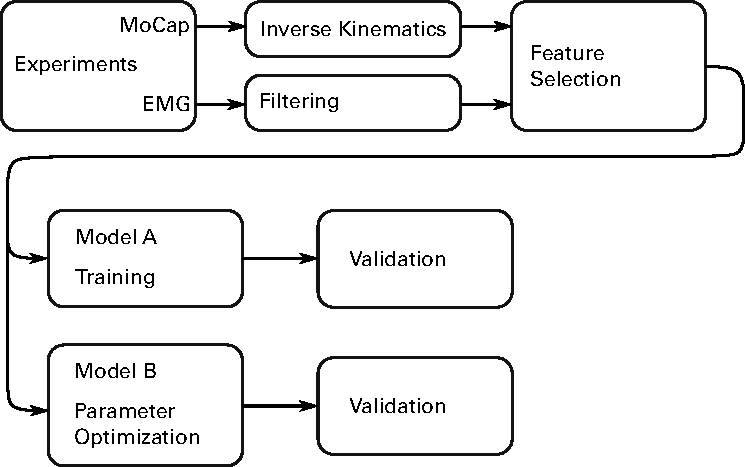
\includegraphics[width=0.8\textwidth]{images/summer_school_study/schematitc.pdf}%
  \caption{Schematic workflow of data processing. In experiments, Motion Capture (MoCap) data and EMG signals were recorded. They were processed using inverse kinematics and filtering techniques, respectively. The sizes of the large datasets were reduced by selecting specific features. Those were used as training inputs for the two models A and B. The trained models were validated using a validation dataset that also originated from experiments.}%
  \label{fig:schematitc}%
\end{figure}%
%
This author contributed mainly to the fields of data processing, especially filtering of EMG signals and feature selection, derivation and training of both models, A and B, their validation and the overall programming and visualization of the results. The respective fields are presented more detailed in the following, corresponding sections.

\subsection{Structure of this Chapter}
\Cref{sec:exp_study} gives an overview over the experiments, data processing and feature selection, which resulted in the required datasets. In \cref{sec:study_models}, the two models, A and B are described. Results including the validation of the models and a discussion are given in \cref{sec:evaluation}. A conclusion follows in \cref{sec:study_conclusion}.

\section{Experimental Study}\label{sec:exp_study}

\begin{figure}%
    \centering%
    \def\svgwidth{5cm}%
    \input{images/summer_school_study/summer_school_study.pdf_tex}%
    \caption{Experimental setup for the triceps trials. The subject pulls down a rope over a pulley which is connected to a weight with mass $m_w$.
    Angles required for the kinematic formulation are the elbow angle, $\phi_e$, the forearm angle, $\phi_a$, and the angle of the weight, $\phi_w$. The length of the ulna bone is denoted by $\ell_u$.}%
    \label{fig:summer_school_study}%
\end{figure}%

At first, details about the experimental study are given. Experiments are required to identify the model parameters for the particular subject. First, the experimental setup is described, second, details on the processing of the measured values are given.

\subsection{Experimental Trials}

In a series of experiments, eight different actions of flexing and extending the elbow were performed by the subject. Weights of 3 kg and 5 kg were hold in the hand during the elbow flexion trials. For the elbow extension trials, a pulley system was installed that redirected the force of the weight such that the downward movement of the forearm acted against the direction of the force. This is shown in \cref{fig:summer_school_study}. A detailed description of the experimental trials can be found in \cite{summerschool2019}.

Time series of position and velocity of upper arm and forearm were recorded using a Motion Capture system. It consisted of eight cameras that tracked three markers placed on shoulder, elbow and wrist of the subject. 

The elbow torque, $\tau$, was computed as
\begin{equation*}
  \begin{array}{lll}
    \tau = m_w\,g\,\ell_u\,\sin(\phi_w) - m_{a}\,g\,\dfrac{\ell_u}{2}\,\sin(\phi_a),
  \end{array}
\end{equation*}
where $(m_w\,g)$ is the force of the weight, $m_{a}$ is the mass of forearm and hand, $\ell_u$ is the length of the ulna bone and $\phi_a$ and $\phi_w$ are the angles of the forearm and rope, as visualized in \cref{fig:summer_school_study}.

\subsection{Data Processing}
From the captured data, derived quantities of biceps ($B$) and triceps $(T$) muscles were estimated using a geometric model of the upper arm. 
The geometric model is available in the software OpenSim \cite{OpenSim2007} and was customized for the particular subject. The inverse kinematics module of OpenSim was used to estimate the muscle tendon unit lengths, $\ell_{\text{MTU},M}$, contraction velocities, $v_M=\dot{\ell}_M$ and moment arms $r_{M}$ of the two muscles, $M\in\{B,T\}$.

EMG signals were captured by two electrodes on the skin above the biceps and triceps muscles. For both signals, several preprocessing steps were applied to obtain the inputs for the two models, A and B.
The raw signal was filtered according to the procedure of \cite{Falisse2016}. First a fourth-order Butterworth high pass filter with cutoff frequency of 30 Hz was applied to reduce non-zero average voltages. The resulting signal was full-wave rectified by taking the absolute value of every measured data point. Then, application of a fourth-order Butterworth low pass filter with 10 Hz cutoff frequency yielded a smoothed signal.
The resulting filtered EMG signals were normalized to the interval $[0,1]$, such that the value of 1 corresponds to the experimentally determined value of maximum voluntary contraction.

The measured EMG signals on the skin directly correspond to the electric excitation level in the muscle, $u$. Excitation leads to the release of free calcium ions within the sarcomere. Binding of calcium ions to myosin increases the concentration of cross-bridges, which is commonly known as the muscular activation, $\alpha$. The muscular activation directly corresponds to the produced force of the muscle \cite{Bayer2017}.

The concentration of free calcium ions is denoted as $\gamma$ and can be computed from excitation, $u$, by the following first order differential equation \cite{Hatze1977},
%
\begin{equation*}
  \begin{array}{lll}
    \dot{\gamma} = m\,(u - \gamma).
  \end{array}
\end{equation*}
%
We used the filtered EMG signal, $u$, to obtain values for $\gamma$. \Cref{fig:emg_filtering} shows the raw and filtered EMG signals and the resulting free calcium concentration for a sample of the experimental data.

\begin{figure}%
  \centering%
  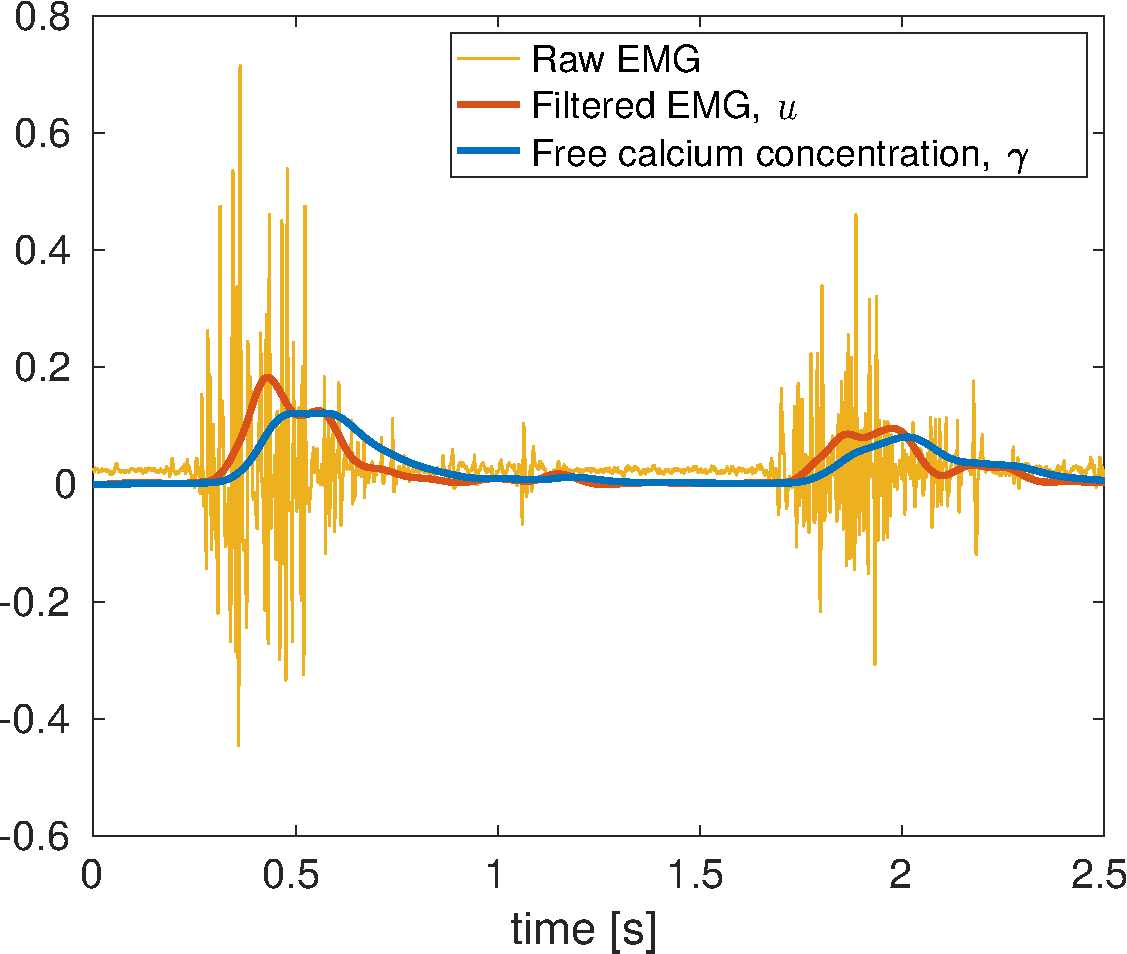
\includegraphics[width=0.8\textwidth]{images/summer_school_study/emg_filtering.pdf}%
  \caption{From raw EMG data of the biceps (yellow) to the filtered signal, $u$, (red) to the free calcium concentration, $\gamma$ (blue). The data is taken from the beginning of the first ellbow flexion experiment. It can be seen that the filtering smooths out the initial signal and removes the constant offset. The free calcium ion concentration follows the filtered EMG with a short delay.}%
  \label{fig:emg_filtering}%
\end{figure}%

The activation of the muscle, $\alpha$, does not only depend on the free ion concentration, $\gamma$, but also on the current state of muscle contraction. This excitation-contraction coupling has to be described by a dynamic system of ODEs and is included in model B.
Therefore, preprocessing is completed with computing the free calcium concentration $\gamma$ and not the activation $\alpha$.

The experimental trials were split into $n_\text{trials}=7$ experiments to be used for model identification and one for validation.
The total captured number of values in the training experiments, $N$, was too large, such that not all points could be used for training of models A and B.
To reduce the amount of data and, thus, speed up the computation, we selected $n \ll N$ featured values with the aim that they are representative for the whole data set.
For every experimental trial, we choose the same fixed number of data points, $n_\text{per\_trial}$.
Our selection algorithm identifies $n_\text{per\_trial}$ time steps, $t_i, i=1, \dots, n$ such that the summed values of the free calcium concentrations for biceps and triceps, $\gamma_B(t_i) + \gamma_T(t_i)$, are evenly distributed along the value range.
This leads to $n = n_\text{trials} \cdot n_\text{per\_trial}$ selected data points.

The set of training data $\mathcal{D} = \mathcal{X} \times \mathcal{Y}$ consists of the $n$ selected vectors of the experimental values that are the input to the system of muscles, $\bfx_i \in \mathcal{X}, i=1,\dots, n$, together with the observed output values, $y_i \in \mathcal{Y}, i=1,\dots,n$.
The input vectors contain values for muscle tendon unit lengths, contraction velocities, moment arms and free calcium ion concentrations for biceps and triceps each, $\bfx_i = (\ell_{\text{MTU},B}, \ell_{\text{MTU},T}, v_B, v_T, r_{B}, r_{T}, \gamma_B, \gamma_T)^\top(t_i)$. The output values consist of the elbow torques, $y_i = \tau(t_i)$. This data set, $\mathcal{D}$, serves as training input for both models A and B.

\section{Models}\label{sec:study_models}

The current section describes the two model approaches that can predict elbow torques from experimental input data. \Cref{sec:data_driven_model} introduces the non-parametric data driven model, A. Afterwards, \cref{sec:biophysical_model} presents the biophysically based model, B. It requires a parameter optimization, which will be described in \cref{sec:parameter_optimization}.

\subsection{Data-driven Model A}\label{sec:data_driven_model}

The first modeling approach uses a non-parametric model. Such model approximates the function $f$ that maps from input to output data points. The function $f$ is learned by using the training data sets. Regression is used to obtain predictions for new data points. In our case, we use a propabilistic model that considers the propability distribution of the model function.

We use the method of \emph{Gaussian Process Regression}. A Gaussian process is a collection of random variables such that the joint distribution of every finite subset of these random variables is multivariate normal (Gaussian).
In our example, each input data point in the space of measured values, $\bfx \in \mathcal{X}$ has an associated random variable $f(\bfx)$ that describes the output of the model for this point.

A Gaussian process, $\mathcal{GP}$, is characterized by a mean function, $m(\bfx)$, and a kernel function, $k(\bfx,\bfx')$ that models the covariance between any pair of points, $\bfx, \bfx' \in \mathcal{X}$. Different choices of kernel functions are possible and can depend on hyperparameters, $\bfpsi$. Describing observed values, $y$, by a Gaussian process distribution can be expressed as
\begin{equation*}
  \begin{array}{lll}
    y \sim \mathcal{GP}\big(m(\bfx), k(\bfx,\bfx',\bfpsi)\big).
  \end{array}
\end{equation*}
This representation is non-parametric in the sense that no particular parametric form of the function $y=f(\bfx)$ is assumed whose parameters would be determined. Instead, the probabilistic model is constructed using the observed function values at measured inputs, $\bfx \in \mathcal{X}$.
%More specifically, the conditional distribution $p(y|\bfx)$ considered.

Gaussian Process Regression is based on \emph{Bayesian Inference} to update a prior belief of the model to a posterier model using information contained in observations of the process.
The observed data is the set of measurements, $\mathcal{D}$. 

The \emph{prior} distribution, $p(\bff\mid\mathcal{X},\bfpsi)$, is described by the Gaussian process as 
\begin{equation*}
  \begin{array}{lll}
    p(\bff\mid\mathcal{X},\psi) = \mathcal{N}(\bff\mid\bfm,\bfK),
  \end{array}
\end{equation*}
with mean values $\bfm = (m(\bfx_i))^\top_{i=1,\dots,n}$ and convariance matrix $\bfK$ with $K_{ij} = k(\bfx_i,\bfx_j,\bfpsi).$

The \emph{likelihood}, $p(\bfy\mid f(\bfx), \bftheta)$, describes the probability of an observation $\bfy$ given a particular model, $f$. The vector $\bftheta$ denotes additional parameters of the likelihood. 

Using Bayes' rule, the \emph{posterior} distribution, $p(\bff\mid\mathcal{D})$, of the function values, $\bff$, can be computed from prior and likelihood as
\begin{equation*}
  \begin{array}{lll}
    p(\bff\mid\mathcal{D},\bftheta,\bfpsi) 
      = \dfrac{p(\bfy\mid\bff,\bftheta)\,p(\bff\mid\mathcal{X},\bfpsi)}{p(\mathcal{D}\mid\bftheta,\bfpsi)}.
  \end{array}
\end{equation*}
This results in a measure for the uncertainty of the model, $f$, at unobserved points $\bfx_\ast \notin \mathcal{D}$. 

Additionally, the fact that the measured quantities in the experiments are subject to measurement noise can be incorporated into the model.
The assumption $y = f(\bfx) + \eps$ adds a normally distributed value of observational noise, $\eps \sim \mathcal{N}(0,\sigma_n^2)$, to the formulation. The noise variance, $\theta = \sigma_n^2$, is an additional parameter of the likelihood. 

It is also possible to explicitly model the mean function, $m(\bfx)$. By relacing the model $f(\bfx)$ by
\begin{equation*}
  \begin{array}{lll}
    g(\bfx) = f(\bfx) + \bfh(\bfx)^\top \bfbeta,
  \end{array}
\end{equation*}
we allow for a global trend in the data that is formulated in terms of a vector of explicit basis functions, $\bfh(\bfx)$, and corresponding coefficients, $\bfbeta$.

The algorithm for Gaussian Process Regression involves estimating several values from the given data. The hyperparameters of the covariance function, $\bfpsi$, the noise variance, $\bftheta$, and the coefficients of the fixed basis functions, $\bfbeta$, are determined by solving an optimization problem. The computation involves matrix inversions and has a computational complexity that is cubic in the number of data points, $\O(n^3)$. For details, the reader is referred to the literature \cite{Rasmussen2005,kuss2006gaussian}.

%$p(\bff^\ast | \mathcal{D},\mathcal{X}^\ast)$
\subsection{Biophysical Model B}\label{sec:biophysical_model}

During elbow flexion, three muscles are involed: biceps brachii, brachialis and brachioradialis. For simplicity, only biceps brachii, which contributes most, is considered is the current study, the effects of the other two muscle are lumped and contained in the biceps brachii model.

Thus, the biophysical model consists of two Hill-type muscle models, for biceps and triceps, respectively. The muscle models are arranged around a hinge joint for the elbow angle. The muscle forces contribute to the torque at the elbow over their respective moment arms.

Hill-type models describe the macroscopic, dynamic mechanical behaviour of an entire muscle along a one-dimensional line of action.
The behaviour is formulated by mathematical functions that have to be parameterized to fit experimental observations.

%Such models are often used to compute muscle forces in simulations of various movements, e.g. \cite{Siebert2003}, \cite{Kistemaker2006}.
Multiple variants of Hill-type models exist that use various configurations of mechanical elements to consider different effects of the muscle. The original model was proposed in \cite{Hill1938}. It contains a contractile element (CE) and two elastic elements, arranged in series and in parallel to the CE.
The authors of \cite{Siebert2008} compare two different approaches using these three elements. The effect of tension in eccentric contractions is added to the Hill-type model by \cite{Till2008}. The authors of \cite{Gunther2007} add a forth, damping element to account for high-frequency damping of the muscle tissue. In \cite{Morl2012}, electro-mechanical delay is investigated with and without the additional damping element. 

\begin{figure}%
  \centering%
  \def\svgwidth{0.5\textwidth}
  \input{images/summer_school_study/hilltype.pdf_tex}%
  \caption{Mechanical structure of the Hill-type muscle model. The force generating contractile element (CE) is parallel-connected to the parallel elastic element (PEE) and connected in series to a second parallel-connected structure of the serial elastic element (SEE) and the serial damping element (SDE). The length of the whole muscle tendon unit, $l_\text{MTU}$, is composed of the common length of CE and PEE, $l_\text{CE}$, and the common length of SEE and SDE, $l_\text{SEE}$. The variable $l_\text{CE}$ is an internal state of the model.}
  \label{fig:hilltype}%
\end{figure}%

\newcommand{\CE}{\text{CE}}
\newcommand{\MTU}{\text{MTU}}

We employ the four-element Hill-type muscle model that is described by \cite{Hilltype2014}. The structure is visualized in \cref{fig:hilltype}. It consists of four components: the contractile element (CE), the parallel elastic element (PEE), the serial elastic element (SEE) and the serial damping element (SDE). Inputs to the model are the muscular activation, $\alpha(t)$, and length and contraction velocity of the muscle tendon unit (MTU), $l_\MTU(t)$ and $\dot{l}_\MTU(t)$.
The output of the model is the muscle force, $f_\text{MTU}(t)$. The model contains one internal state variable, the length of the CE, $l_\text{CE}(t)$. The muscle dynamics determine this internal length and its time derivative, the contraction velocity of the CE, $\dot{l}_\text{CE}(t)$.

The force of the MTU is computed as sum of the forces of the respective parallel elements as visualized in \cref{fig:hilltype},
\begin{equation}\label{eq:hill_type0}
  \begin{array}{lll}
    F_\MTU = F_\CE(l_\CE, \dot{l}_\CE, \alpha) + F_\text{PEE}(l_\CE) = F_\text{SEE}(l_\CE,l_\MTU) + F_\text{SDE}(l_\CE,\dot{l}_\CE,\dot{l}_\MTU,\alpha).
  \end{array}
\end{equation}
The force terms of the four elements, $F_\CE, F_\text{PEE}, F_\text{SEE}$ and $F_\text{SDE}$ are described by analytical functions that use a total of 19 parameters. The second identity of \eqref{eq:hill_type0} can be solved for $\dot{l}_\CE$ to get an evolution equation for the length of the CE, $l_\CE$, which is an internal state of the model. Together with the activation dynamics, which describes the relation between the free calcium ion concentration, $\gamma$, and the muscle activation, $\alpha \in [0,1]$, we get the following coupled system of differential-algebraic equations,
\begin{align}
  F_\MTU &= F_\MTU(l_\MTU,l_\CE,\dot{l}_\CE,\alpha),      \label{eq:hill_type1} \\[4mm]
  \dot{l}_\CE &= f_\CE(l_\CE,l_\MTU,\dot{l}_\MTU,\alpha), \label{eq:hill_type2}\\[4mm]
  \alpha &= f_\alpha(\gamma, l_\CE).                      \label{eq:hill_type3}
\end{align}
The detailed equations of the force terms in \cref{eq:hill_type1,eq:hill_type2} can be found in \cite{Hilltype2014}. \Cref{fig:force_curves_generic} visualizes characteristic curves of the model. \Cref{fig:force_curves_generic_length} shows how the generated force depends on the length of the CE. The active force, shown by the solid red line, has its maximum at an optimal length, $l_\text{CE,opt}$. This is explained by the exposure of the actin and myosin filaments in the sarcomere relative to each other, which is lower when the actin filaments are pulled apart or pushed together.
The dashed line in \cref{fig:force_curves_generic_length} represents the passive force of the elastic muscular tissue which is essentially generated by the titin proteins in the sarcomere. Only starting from a certain length, the structure excerts reaction forces against lengthening forces to avoid overstretching of the muscle.

The force-velocity relation of the Hill-type model is shown in \cref{fig:force_curves_generic_velocity}. The curve is composed of two branches: 
The concentric branch for shortening contraction with $\dot{l}_\CE \leq 0$ and the eccentric branch for lengthening contraction with $\dot{l}_\CE > 0$. It can be seen that the generated force increases monotonically over the lengthening velocity. It approaches a limit for maximum positive and negative velocity. These limits are given by parameters and are exemplary for how the shape of the curves of a Hill-type model can be parametrized.

\begin{figure}%
  \centering%
  \begin{subfigure}[t]{0.9\textwidth}%
    \centering%
    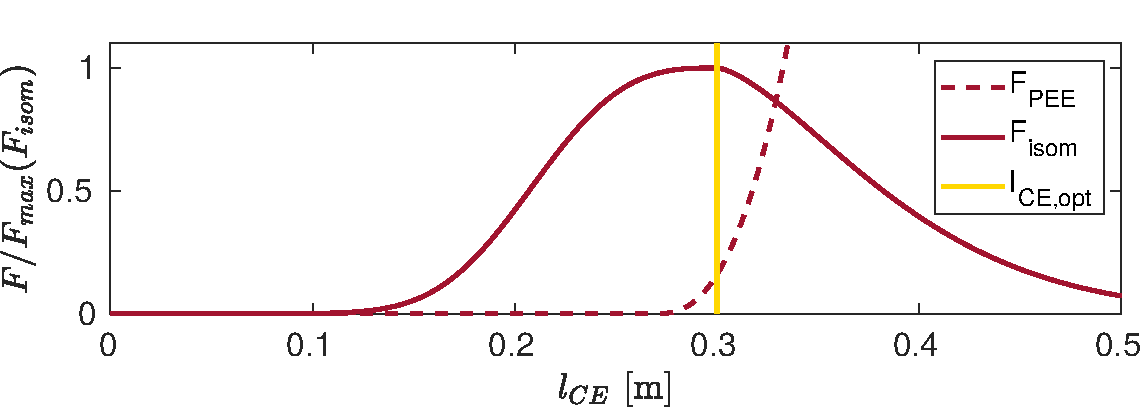
\includegraphics[width=\textwidth]{images/summer_school_study/force_curves_generic_length.pdf}%
    \caption{Force-length curves of the PEE (dashed red line) and CE (solid red line), for isometric condition ($\dot{l}_\CE=0$) and normalized to the maximum isometric force. The optimal length of the CE, $l_\text{CE,opt}$, is shown as yellow vertical line. The force of the PEE, $F_\text{PEE}(l_\CE)$, is zero for $l_\CE < 0.9\,l_\text{CE,opt}$. The isometric contraction force, $F_\text{isom} = F_\CE(l_\CE)$ is formulated by two branches for separated by $l_\text{CE,opt}$.}%
    \label{fig:force_curves_generic_length}%
  \end{subfigure}\\[6mm]
  \begin{subfigure}[t]{0.9\textwidth}%
    \centering%
    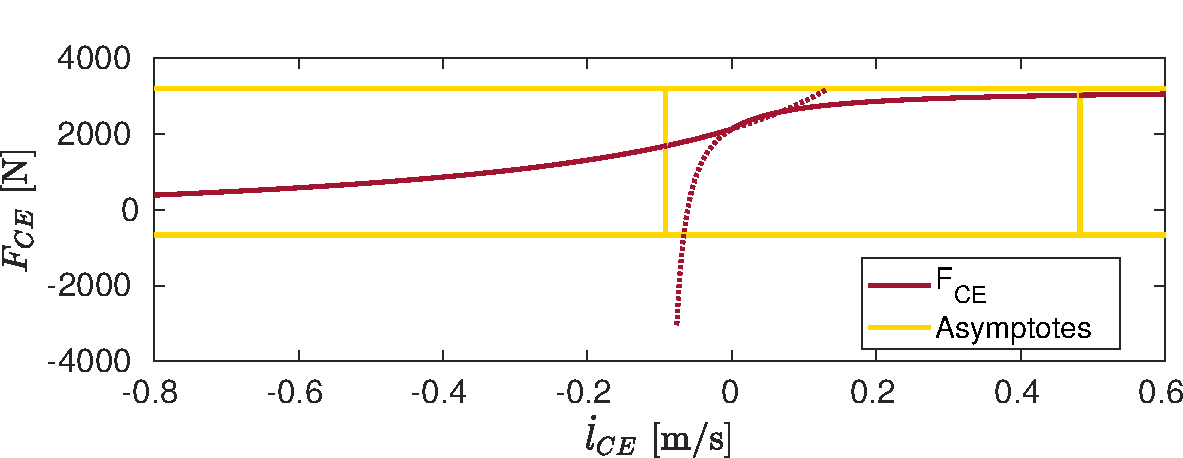
\includegraphics[width=\textwidth]{images/summer_school_study/force_curves_generic_velocity.pdf}%
    \caption{Force-velocity curve of the CE, $F_\CE(\dot{l}_\CE)$, at optimal length, $l_\CE=l_{\CE,\text{opt}}$, and for activation level $\alpha=0.5$. The function (red solid line) is formulated piecewise, the base functions of the two branches are shown as red dotted lines. Their limits are visualized by the yellow horizontal and vertical asymptotes.}%
    \label{fig:force_curves_generic_velocity}%
  \end{subfigure}%
  \caption{Force-length and Force-velocity relations for the muscle model with generic parameters taken from literature \cite{Hilltype2014}.}%
  \label{fig:force_curves_generic}%
\end{figure}%

The model of activation dynamics, \cref{eq:hill_type3}, is the one of Hatze et al. \cite{Hatze1977} with parameters taken from \cite{Bayer2017}.

\subsection{Parameter Identification for Model B}\label{sec:parameter_optimization}

The process of model identification finds the parameters that make the model B predict correct values for the specific subject. An optimization scheme finds the parameters that minimize the error in the predicted outcome for the training data set.

The following minimization is performed,
\begin{align}
  &&\min\limits_{\substack{\bftheta_M,l_{\CE,M}(t), \\M \in \{B,T\}, \,t \in \mathcal{T}}} &\sum\limits_{t\in \mathcal{T}}|\tau(t) - \hat{\tau}(t)|^2
   \label{eq:opt_1}\\[4mm]
  &&\text{s.t. }\forall t \in \mathcal{T}:\quad &\tau(t) = F_{\MTU,B}(t,l_{\CE,B},\bftheta_B) \cdot \hat{r}_B(t) \notag\\
      &&&\qquad\quad- F_{\MTU,T}(t,l_{\CE,T},\bftheta_T) \cdot \hat{r}_T(t),                 \label{eq:opt_2}\\[4mm]
  &&& \dot{l}_{\CE,M}(t) = \dot{\hat{l}}_{\MTU,M}(t),\quad M \in \{B,T\},      \label{eq:opt_3}\\[4mm]
  &&& \bftheta_B, \bftheta_T \in \Theta,                                       \label{eq:opt_4}\\[4mm]
  &&& l_{\CE,M}(t) \in [0,l_{\MTU,M}(t)],\quad M \in \{B,T\}.                  \label{eq:opt_5}
\end{align}

The optimization variables are the parameters for the biceps and triceps Hill-type models, $\bftheta_B$ and $\bftheta_T$, and the lengths of the contractile elements for both models at every point in time, $l_{\CE,B}$ and $l_{\CE,T}$. The variables designated as $\hat{\square}$ are the measured quantities from the training experiments. The objective function, \Cref{eq:opt_1}, penalizes the difference between computed torque, $\tau$, and measured torque, $\hat{\tau}$, at every timestep of the training data, $t \in \mathcal{T}$. The torque is computed in \cref{eq:opt_2} by multiplying the predicted forces, $F_{\MTU,B}, F_{\MTU,T}$, with the measured moment arms, $\hat{r}_B, \hat{r}_T$.

In \cref{eq:opt_3}, the contraction velocities are constraint to the measured values. Because the lengthening velocity of the CE, $\dot{l}_\CE$, is an internal quantity and, thus, cannot be observed in experiments, we assume it to be equal to the lengthening velocity of the whole muscle, $\dot{l}_\CE \approx \dot{l}_{\MTU} = \dot{l}_\text{CE} + \dot{l}_\text{SE}$. This requires the assumption $\dot{l}_{\text{SE}} \approx 0$ which can be justified given the low dynamic nature of the experiments.

By \cref{eq:opt_4} we bound each of the parameters, $\bftheta_B,\bftheta_T$, to a range between half and twice the generic value from literature.
The lengths of the CEs are constraint by \cref{eq:opt_5} to be positive and smaller than the length of the MTU.

All optimization variables are normalized to improve the numeric conditioning of the optimization problem. 
The parameters $\bftheta_B,\bftheta_T$ are normalized with respect to generic values from literature, that were taken from \cite{Gunther2007, Morl2012, Hilltype2014}. The initial values are set to these generic parameters, which corresponds to the value one for the normalized variables.
The internal states, $l_{\CE,B},l_{\CE_T}$, are normalized with respect to the measured MTU lengths, $\hat{l}_{\MTU,B}, \hat{l}_{\MTU,T}$ and initialized to zero.

\section{Results and Discussion}\label{sec:evaluation}

In the following, results of combining the experimental data with the two models, A and B are presented.
At first, \cref{sec:res_feature_selection} gives details on the preprocessed data. The training phase is described in \cref{sec:res_training}. Applying the trained models to the validation data is done in \cref{sec:res_validation}. For model A, \cref{sec:res_simplified_a} tests a simplified version. For model B, \cref{ref:res_insights_b} shows some insights into the optimized parameter values.

\subsection{Feature Selection}\label{sec:res_feature_selection}
% intro
The experimental data is split into a training and a validation dataset. \Cref{fig:selected_points} shows the processed data of the training data set. In total we captured $N=34,934$ data points for the seven experimental trials. Out of these, we select $n_\text{per\_trial}=40$ feature points in every trial, leading to a total of $n=n_\text{per\_trial}\cdot n_\text{trials}=280$ points. The selected points are visualized by crosses in the top plot of \cref{fig:selected_points}. It can be seen that the algorithm distributes the feature points equally along the $\gamma$ axis.

\begin{figure}%
  \centering%
  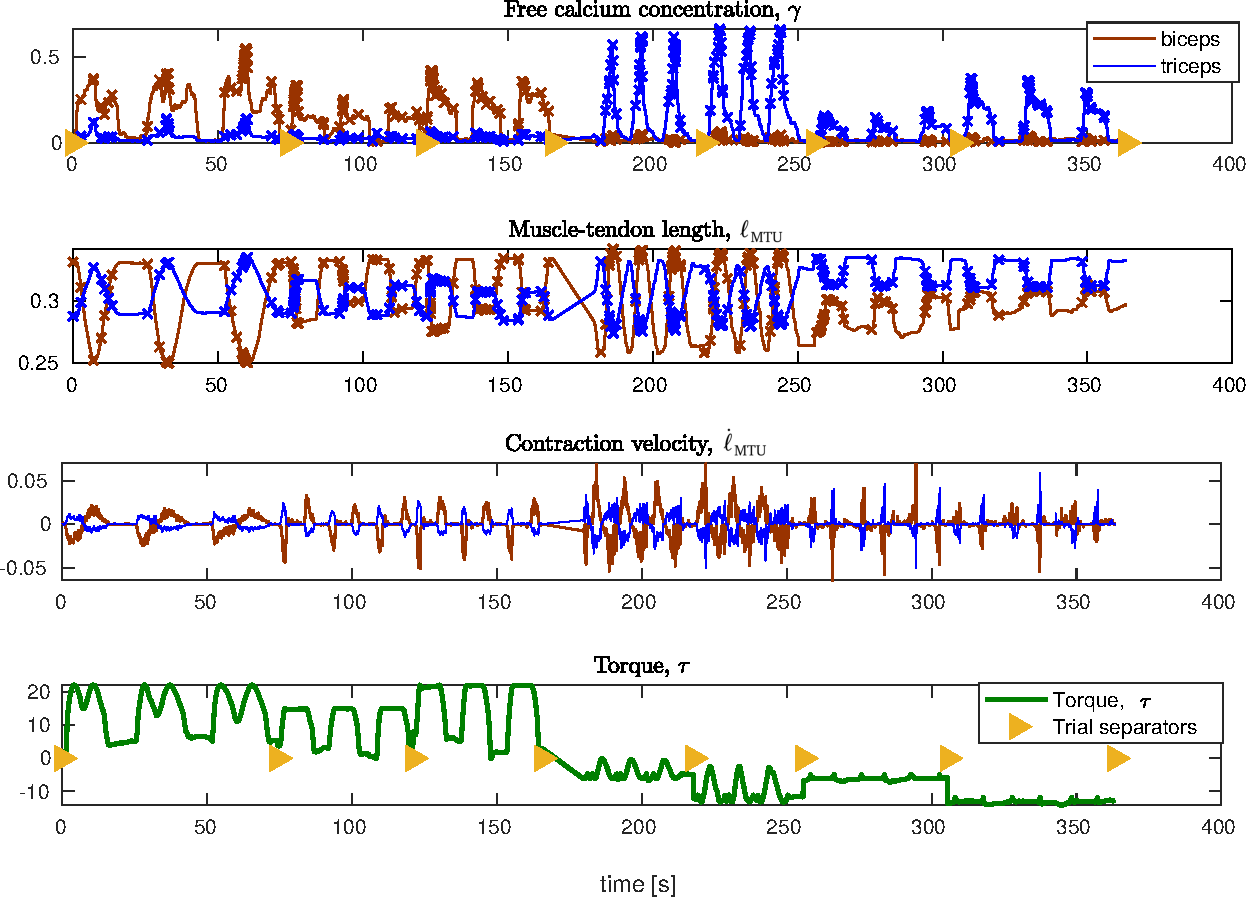
\includegraphics[width=\textwidth]{images/summer_school_study/selected_points.pdf}%
  \caption{Processed experimental values over time that were used for training of both models. The concatenated data of seven trials is shown which yields a total end time of 363.32 s. The individual trials are separated by the yellow triangles on the $x$-axis. The three upper plots show the values of $\gamma, l_\MTU$ and $\dot{l}_\MTU$ for both biceps (brown) and triceps (blue), the bottom plot shows the elbow torque, $\tau$. The selected feature points are visualized as crosses in the two top plots. In the upper-most plot, it can be seen that the first three trials, which correspond to elbow flexion, mainly activated the biceps muscle, whereas in the last four trials, corresponding to elbow extension, the triceps is more active.
}%
  \label{fig:selected_points}%
\end{figure}%

\subsection{Training of the Models}\label{sec:res_training}

Training of the Gaussian Process of model A was performed using the ready to use implementation provided by MATLAB.
We parametrized the covariance by a squared exponential kernel and used constant basis functions, $H(x) = 1$. We enabled observational noise, its standard deviation, $\sigma_n^2$, was found by optimization during training of the model.

For training of model B, the optimization problem for the parameters needed to be solved. We implemented the Hill-type models and the constraints also in MATLAB and used the nonlinear programming implementation, \code{fmincon}, to minimize the given bounded and nonlinear constrained, multivariable function.

The total number of optimization variables can be computed by $2\cdot 19 + 2n = 598$, as each of the parameter vectors $\bftheta_B,\bftheta_T$ had 19 entries. The resulting parameter values and their relation to the initial values are summarized in \cref{tab:model_b_parameters}. It can be seen that none of the final parameter values are limited by the constraints which would be $-50\%$ and $+100 \%$. However, setting the constraints helps the optimizer to stay in the valid range of meaningful model parameters.

\begin{table}[t] 
  \centering
  %\begin{scriptsize}
  
    \begin{tabular}{@{}llllll@{}}
%\hline
 %| param              | biceps   |            | triceps  |            %|
 %| ------------------ | -------- | ---------- | -------- | ---------- %|
 %| CE_F_max           | +11.03 % | 4729.97    | -49.04 % | 2171.04    |
 %| CE_l_CEopt         | +31.72 % | 0.40       | -25.36 % | 0.22       |
 %| CE_DeltaW_limb_des | +10.86 % | 0.39       | +10.86 % | 0.39       |
 %| CE_DeltaW_limb_asc | +91.61 % | 0.67       | +5.05 %  | 0.37       |
 %| CE_v_CElimb_des    | +10.86 % | 1.66       | +10.86 % | 1.66       %|
 %| CE_v_CElimb_asc    | -46.39 % | 1.61       | +95.87 % | 5.88       |
 %| CE_A_rel0          | +14.03 % | 0.29       | -20.34 % | 0.20       |
 %| CE_B_rel0          | +77.51 % | 3.99       | +41.38 % | 3.18       |
 %| CE_S_eccentric     | -4.12 %  | 1.92       | +22.92 % | 2.46       |
 %| CE_F_eccentric     | -30.94 % | 1.04       | +36.79 % | 2.05       |
 %| PEE_L_PEE0         | +10.86 % | 1.00       | +10.86 % | 1.00       |
 %| PEE_l_PEE0         | +10.86 % | 0.30       | +10.86 % | 0.30       |
 %| PEE_v_PEE          | +10.86 % | 2.77       | +10.86 % | 2.77       |
 %| PEE_F_PEE          | +10.86 % | 2.22       | +10.86 % | 2.22       |
 %| PEE_K_PEE          | +10.86 % | 1410470.38 | +10.86 % | 1410470.38 |
 %| SDE_D_SE           | +10.86 % | 0.33       | +10.86 % | 0.33       |
 %| SDE_R_SE           | +8.63 %  | 0.01       | -10.99 % | 0.01       |
 %| SDE_d_SEmax        | +8.41 %  | 513.16     | -10.64 % | 422.98     |
 %| SEE_l_SEE0         | -24.95 % | 0.13       | -10.28 % | 0.15       |
 %| SEE_DeltaU_SEEnll  | +59.16 % | 0.07       | +23.58 % | 0.05       |
 %| SEE_DeltaU_SEEl    | +63.34 % | 0.03       | +19.02 % | 0.02       |
 %| SEE_DeltaF_SEE0    | -42.40 % | 327.16     | +64.75 % | 935.78     |
 
% contractile element (CE)
%===========================
%  CE_F_max                         % F_max in [N] for Extensor (Kistemaker et al., 2006)
%  CE_l_CEopt                       % optimal length of CE in [m] for Extensor (Kistemaker et al., 2006)
%* CE_DeltaW_limb_des = 0.35;       % width of normalized bell curve in descending branch (Moerl et al., 2012)
%* CE_DeltaW_limb_asc = 0.35;       % width of normalized bell curve in ascending branch (Moerl et al., 2012)
%* CE_v_CElimb_des = 1.5;           % exponent for descending branch (Moerl et al., 2012)
%  CE_v_CElimb_asc = 3.0;           % exponent for ascending branch (Moerl et al., 2012)
%* CE_A_rel0 = 0.25;                % parameter for contraction dynamics: maximum value of A_rel (Guenther, 1997, S. 82)
%* CE_B_rel0 = 2.25;                % parameter for contraction dynmacis: maximum value of B_rel (Guenther, 1997, S. 82)
%  eccentric force-velocity relation:
%* CE_S_eccentric  = 2;             % relation between F(v) slopes at v_CE=0 (van Soest & Bobbert, 1993)
%  CE_F_eccentric  = 1.5;           % factor by which the force can exceed F_isom for large eccentric velocities (van Soest & Bobbert, 1993)

% paralel elastic element (PEE)
%===============================
%  PEE_L_PEE0   = 0.9;                               % rest length of PEE normalized to optimal lenght of CE (Guenther et al., 2007)
%  PEE_v_PEE    = 2.5;                               % exponent of F_PEE (Moerl et al., 2012)
%  PEE_F_PEE    = 2.0;                               % force of PEE if l_CE is stretched to deltaWlimb_des (Moerl et al., 2012)

% serial damping element (SDE)
%=============================
%* SDE_D_SE    = 0.3;               % xxx dimensionless factor to scale d_SEmax (Moerl et al., 2012)
%* SDE_R_SE    = 0.01;              % minimum value of d_SE normalised to d_SEmax (Moerl et al., 2012)
%  SDE_d_SEmax = SDE_D_SE*(CE_F_max*CE_A_rel0)/(CE_l_CEopt*CE_B_rel0);
                                    % maximum value in d_SE in [Ns/m] (Moerl et al., 2012)

% serial elastic element (SEE)
% ============================
%  SEE_l_SEE0        = 0.172;       % rest length of SEE in [m] (Kistemaker et al., 2006)
%  SEE_DeltaF_SEE0   = 568;         % both force at the transition and force increase in the linear part in [N] (~ 40% of the maximal isometric muscle force)
%  SEE_DeltaU_SEEnll = 0.0425;      % relativ stretch at non-linear linear transition (Moerl et al., 2012)
%* SEE_DeltaU_SEEl   = 0.017;       % relativ additional stretch in the linear part providing a force increase of deltaF_SEE0 (Moerl, 2012)
% 
     \toprule
    \textbf{CE} 
      & $F_{\mathrm{max}}\,[\mathrm{N}]$
      & $l_{\mathrm{CE},opt}\,[\mathrm{m}]$ 
      & $\Delta W_{d} \,[\;]$ 
      & $\Delta W_{a} \,[\;]$ 
      & $\nu_{\mathrm{CE},d} \,[\;]$ \\  \midrule
    Generic & $4260$ & $0.3$ & $0.35$ & $0.35$ & $1.5$  \\ %\hline
    Biceps  & $+11.0\%$ & $+31.7\%$ & $+10.9\%$ & $+91.6\%$ & $+10.9\%$  \\ %\hline
    Triceps & $-49.0\%$ & $-25.4\%$ & $+10.9\%$ & $+5.1\%$ & $+10.9\%$  \\ %\hline 
    \addlinespace[2ex]
    \textbf{CE} 
      &  $\nu_{\mathrm{CE},a} \,[\;]$ 
      & $A_\text{rel,0} \,[\;]$  
      & $B_\text{rel,0} \,[\;]$ 
      & $S_\text{ecc} \,[\;]$ 
      & $F_\text{ecc} \,[\;]$\\  \hline
    Generic & $3.0$ & $0.25$ & $2.25$ & $2$ & $1.5$ \\ %\hline
    Biceps & $-46.4\%$ & $+14.0\%$ & $+77.5\%$ & $-4.1\%$ & $-30.1\%$ \\ %\hline
    Triceps &  $+95.9\%$ & $-20.3\%$ & $+41.4\%$ & $+22.3\%$ & $+36.8\%$ \\ %\hline
    \addlinespace[2ex]
    \textbf{PEE} 
      & $L_{\mathrm{PEE},0} \,[\;]$ 
      & $\nu_{\mathrm{PEE}} \,[\;]$ 
      & $F_{\mathrm{PEE}} \,[\;]$
      \\ \hline
    Generic & $0.9$ & $2.5$ & $2.0$  \\ %\hline
    Biceps & $+10.9\%$ & $+10.9\%$ & $+10.9\%$  \\ %\hline
    Triceps & $+10.9\%$ & $+10.9\%$ & $+10.9\%$  \\ %\hline
    \addlinespace[2ex]
    \textbf{SDE} 
      & $D_{\mathrm{SDE}} \,[\;]$ 
      & $R_{\mathrm{SDE}} \,[\;]$ 
      \\ \midrule
    Generic & $0.3$ & $0.01$    \\ %\hline
    Biceps & $+10.9\%$ & $+8.6\%$   \\ %\hline
    Triceps & $+10.9\%$ & $-11.0\%$  \\ %\hline
    \addlinespace[2ex]
    \textbf{SEE} 
      & $l_{\mathrm{SEE},0}\,[\mathrm{m}]$ 
      & $\Delta F_{\mathrm{SEE},0} \,[\;]$  
      & $\Delta U_{l} \,[\;]$  
      & $\Delta U_{nll}\,[\;]$
      \\ \hline
    Generic & $0.172$ & $0.0425$ & $0.017$ & $568$ \\ %\hline
    Biceps & $-25.0\%$ & $-42.4\%$ & $+63.3\%$ & $+59.2\%$ \\ %\hline
    Triceps & $-10.3\%$ & $+64.75\%$ & $+19.0\%$ & $+23.6\%$ \\ %\hline
    \bottomrule
  \end{tabular}

  \caption{Hill-type muscle model parameters of the four elements, CE, PEE, SDE and SEE, initial values given in literature and relative changes of the optimized values. Further explanations of the parameters and references to their initial values are given in \cite{Hilltype2014}.}
  \label{tab:model_b_parameters}
  %\end{scriptsize}
\end{table}

After training of the models A and B using the selected points of the training dataset, both models were tested by a \emph{resubstitution prediction}, i.e. predicting output from the training input data. The results are shown in \cref{fig:measured_optimized_torque_A} for model A and \cref{fig:measured_optimized_torque_B} for model B. As this uses only the selected subset of experimental values, the data points have no natural ordering and therefore were sorted for better visibility.
It can be seen that for both models the predicted value are a good fit to the measured values. For model A, the predicted 95\% confidence interval includes the real values almost everywhere. For model B, the predicted values have a higher variance, especially for high torque values.

\begin{figure}%
  \centering%
  \begin{subfigure}[t]{0.48\textwidth}%
    \centering%
    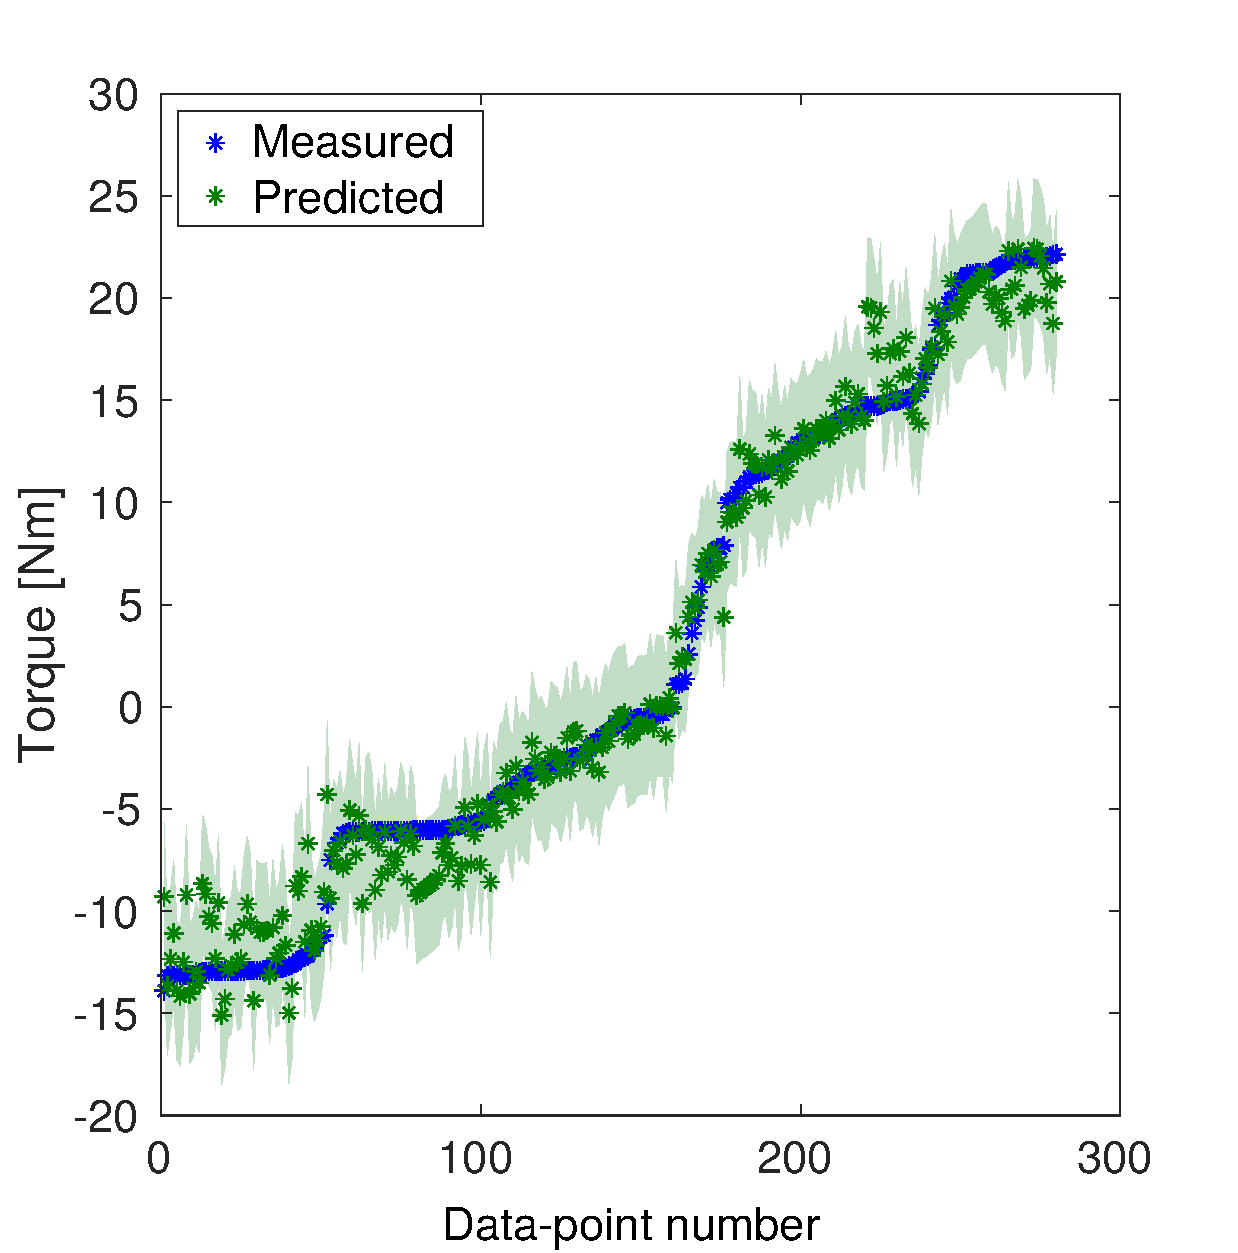
\includegraphics[width=\textwidth]{images/summer_school_study/measured_optimized_torque_A.pdf}%
    \caption{Measured values (blue) and values predicted by Model A (dark green), with 95\% confidence interval (light green).}%
    \label{fig:measured_optimized_torque_A}%
  \end{subfigure}%
  \quad
  \begin{subfigure}[t]{0.48\textwidth}%
    \centering%
    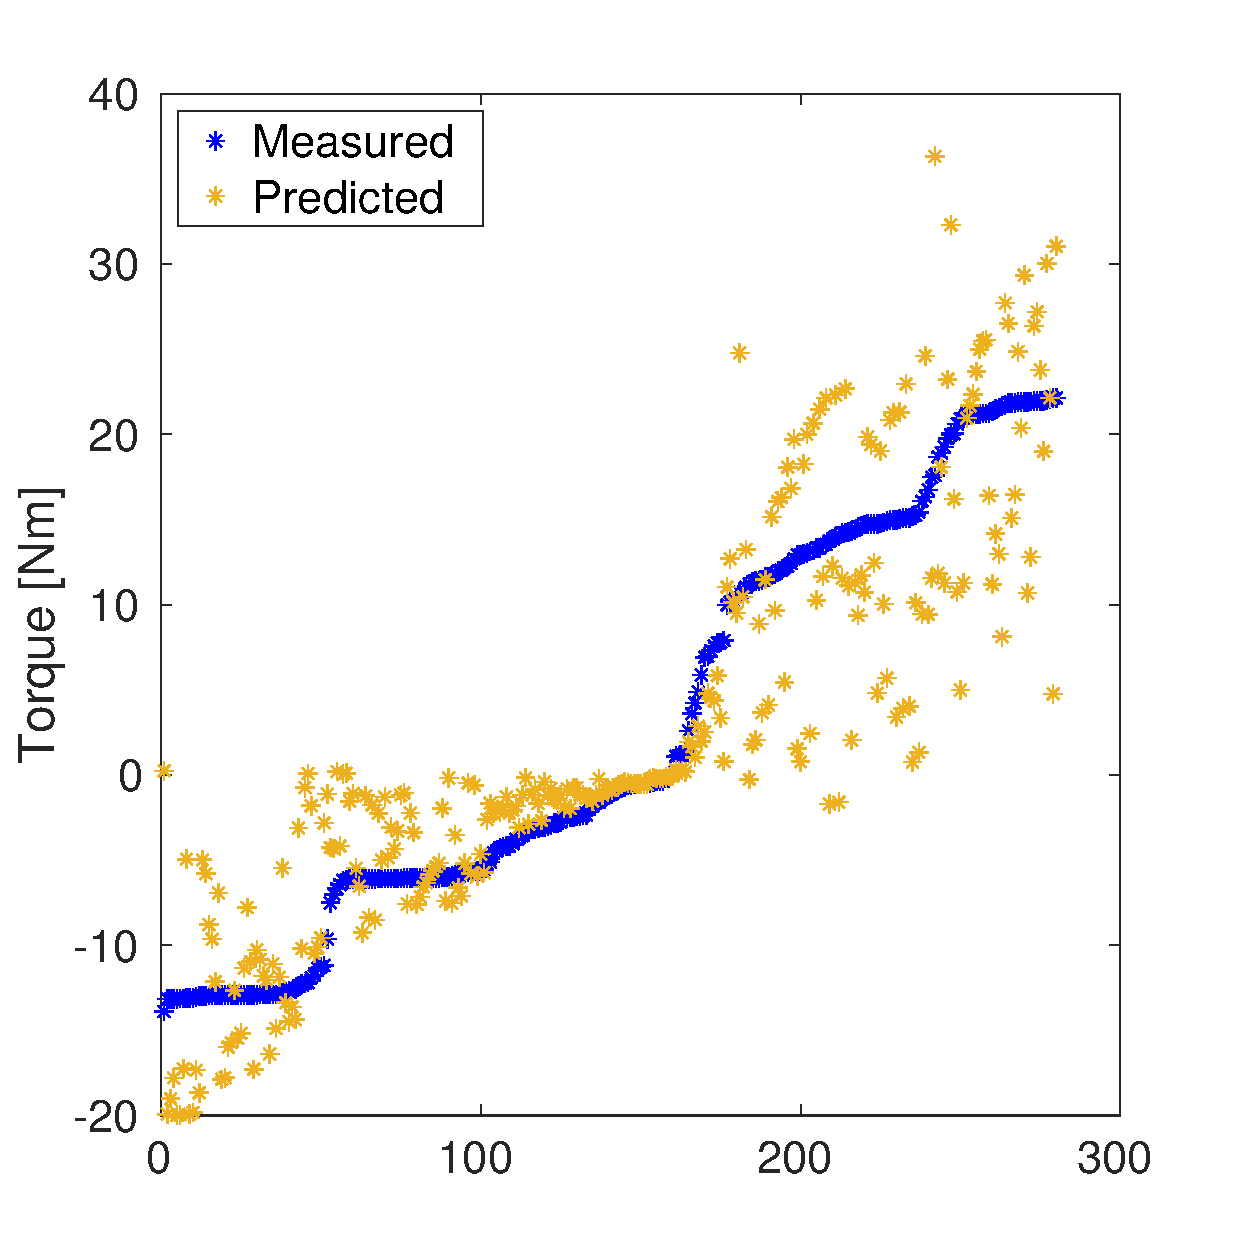
\includegraphics[width=\textwidth]{images/summer_school_study/measured_optimized_torque_B.pdf}%
    \caption{Measured values (blue) and predicted values by Model B (orange).}%
    \label{fig:measured_optimized_torque_B}%
  \end{subfigure}%
  \caption{Measured and predicted torque values for the training data set. The measured points are ordered by magnitude, the order of the predicted points matches the order of the measured points.}%
  \label{fig:measured_optimized_torque}%
\end{figure}%

\subsection{Validation}\label{sec:res_validation}

The next evaluation is to use the validation dataset and compare the predicted outputs of the model with the real, experimental values.
In contrast to the training data, where a small number, $n$, of points was selected, we use all captured values, in total \num{54e3} data points for a time span of $t=54 \si{\second}$. The results are shown in \cref{fig:validation_bv5_40_points}.

\begin{figure}%
  \centering%
  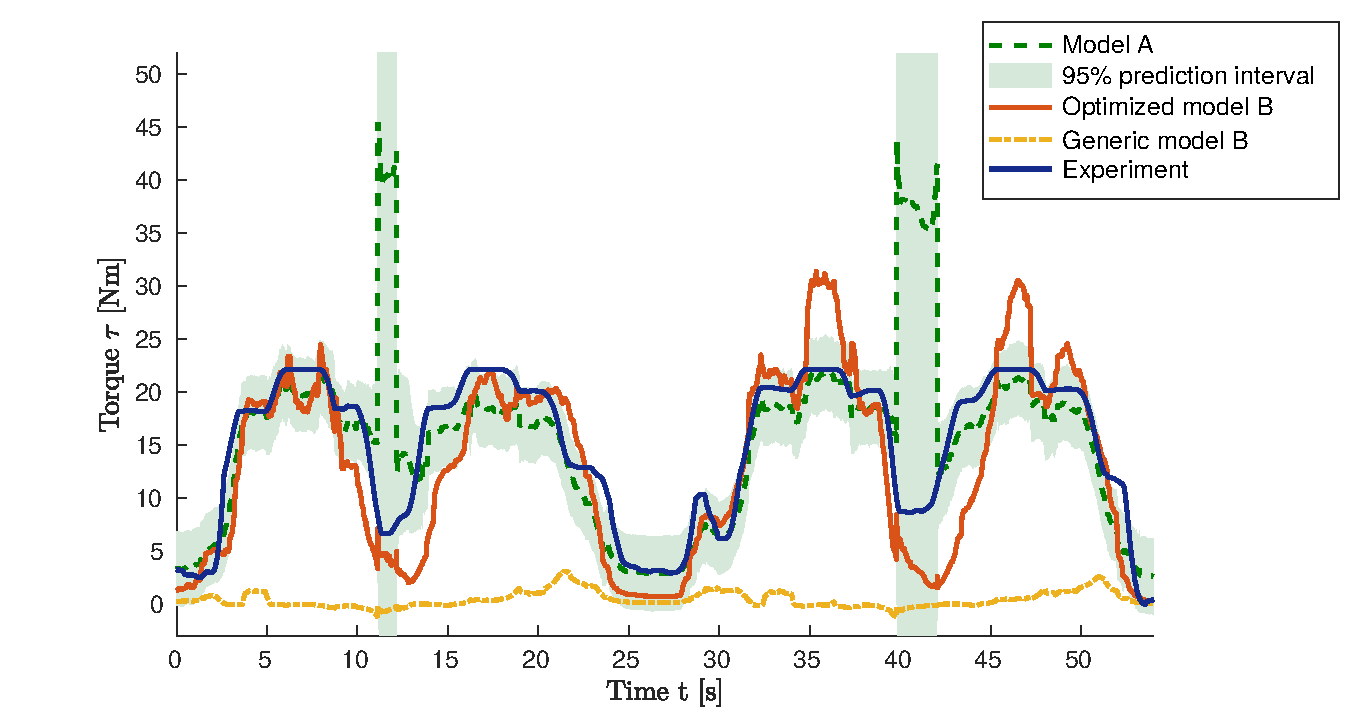
\includegraphics[width=\textwidth]{images/summer_school_study/validation_bv5_40_points.pdf}%
  \caption{Predicted torque values by model A (green), trained model B (red) and untrained model B (yellow), in comparison to the experimentally measured values (blue), for the validation data set.}%
  \label{fig:validation_bv5_40_points}%
\end{figure}%

Comparing the green curve for model A with the blue curve for the experimental data, it can be seen that the predicted values match qualitatively for most of the time span. The predicted torque values are slightly smaller than the real values. Only for the two intervals $[11 \si\second, 12 \si\second]$ and $[40 \si\second, 42 \si\second]$ the predicted value is far off. The 95\% confidence interval that was computed by the Gaussian Process spans a large range for these time intervals which implies that the model prediction is not to be trusted in this area. 

The biophysical model approach, model B was tested in two variants. First, with the generic parameters from literature (yellow curve), second with the subject-specific, optimized parameters (red curve). It can be seen that the generic model fails to predict the torque values whereas the trained model computed reasonable values. These values are worse than most of the predictions from model A, but they succeed in giving a qualitative estimate about a low, medium or high torque output.

The match between models and experiment can be quantified using the normalized root-mean-square error (NRMSE), which is defined as
\begin{equation*}
  \begin{array}{lll}
    \text{RMSE} = \sqrt{\sum\limits_{i=1}^N (\theta_i - \hat{\theta_i})^2 / N},\\[4mm]
    \text{NRMSE} = \dfrac{\text{RMSE}}{\max\limits_i\{\hat\theta_i\} - \min\limits_i\{\hat\theta_i\}}.
  \end{array}
\end{equation*}
The NRMSE for model A is 0.267 which is worse than the value of 0.163 for the trained model B. The generic model B has the worst NRMSE of 0.547.

\subsection{Simplified Model A}\label{sec:res_simplified_a}
An advantage of model approach A is that it forgos any biophysical description and the associated type of model error. It is a generic approach that does not require expert knowledge about the physiological structure. In the present study, however, some level of expert knowledge and physiological model was required in preprocessing the MoCap data, i.e. solving the inverse kinematics of the observed forarm movements to get the kinematic quantities of muscle lengths, velocities and moment arms. Therefore, the next study tries to apply the approach of model A using only the elbow angle instead, which is easier to measure experimentally. Thus, training data consist of input vectors $\bfx_i = (\phi_e(t_i), \gamma_B(t_i), \gamma_T(t_i))^\top \in \mathcal{X}$. In the following, this model is named \say{Simplified model A} in constrast to the \say{Full model A} that used the extended input data.

The results are shown in \cref{fig:measured_optimized_A2}. It can be seen that the resubstitution prediction in \cref{fig:measured_optimized_torque_A2} where the trained model is used to predict the training values shows a perfect fit. In contrast to the full model A, \cref{fig:measured_optimized_torque_A}, here, the learned input-output mapping shows no variance. However, the prediction for the validation dataset in \cref{fig:measured_optimized_torque_A3} shows a high error relative to the experimental data. The curve for the experimental data even lies outside the 95\% confidence interval of the prediction at some points. The NRMSE value has a high value of 0.461. 
The NRMSE values of the full and simplified model A and the generic and optimized model B are summarized in \cref{fig:nrmse}.
This means that simplified model A gives no useful results where the training input is too scarce. Instead, preprocessing of the measurements using a subject specific geometric model, as done for the full model A gives the desired results.

\begin{figure}%
  \centering%
  \begin{subfigure}[t]{0.48\textwidth}%
    \centering%
    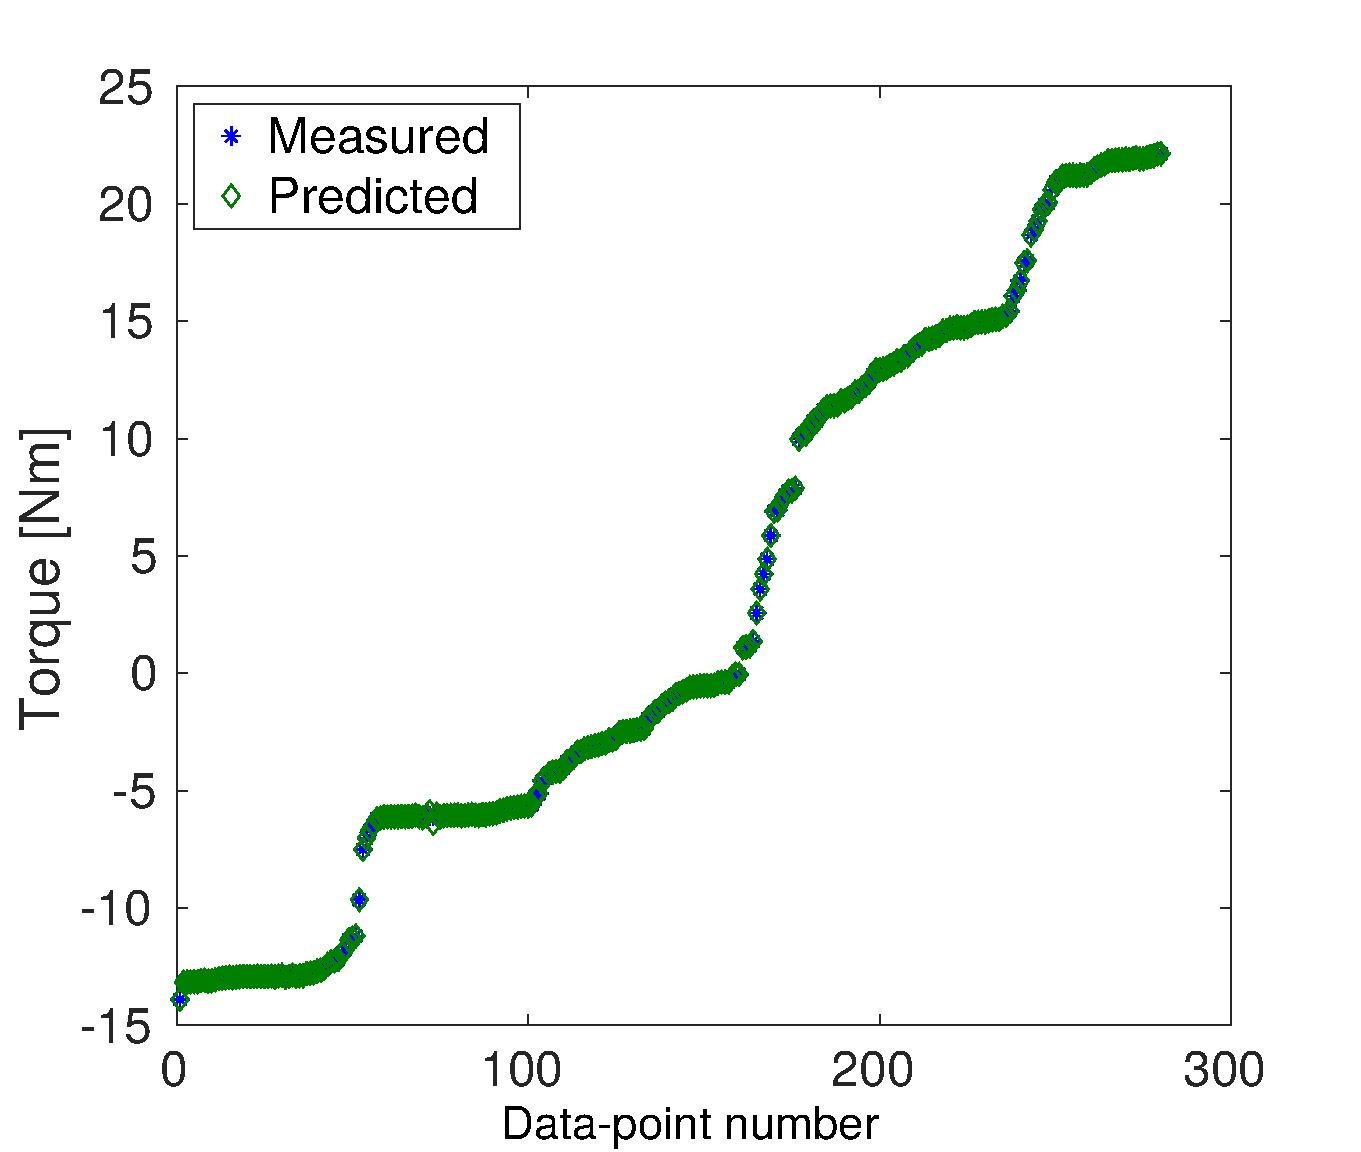
\includegraphics[width=\textwidth]{images/summer_school_study/measured_optimized_torque_A2.pdf}%
    \caption{Measured and predicted torque values of the training dataset, ordered by magnitude. The measured values (blue) and the values predicted by the Gaussian Process (green) lie on each other.}%
    \label{fig:measured_optimized_torque_A2}%
  \end{subfigure}%
  \quad
  \begin{subfigure}[t]{0.48\textwidth}%
    \centering%
    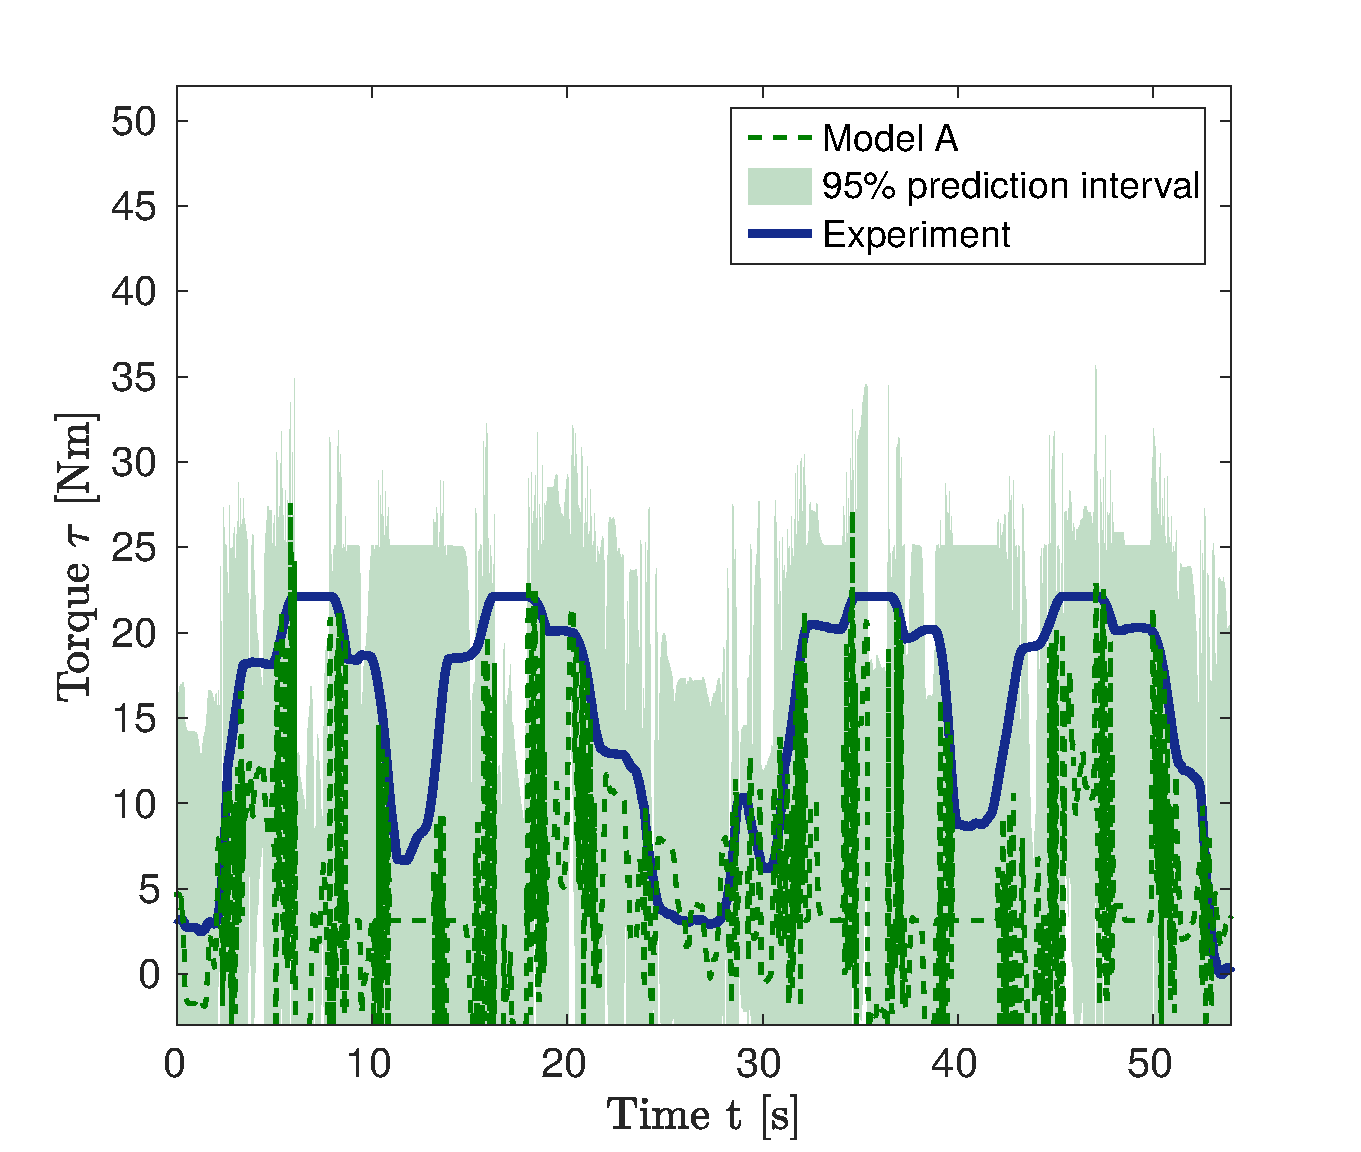
\includegraphics[width=\textwidth]{images/summer_school_study/validation_bv5_40_points_only_gamma_for_training.pdf}%
    \caption{Predicted torque values for the validation trials (green dotted line), 95\% confidence interval (light green) and the reference values of the experiment (blue), which reveal bad prediction capabilities of the simplified model A.}%
    \label{fig:measured_optimized_torque_A3}%
  \end{subfigure}%
  \caption{Result for the simplified model A, where only the elbow angles, $\phi_e$, are used as training input instead of MTU lengths, velocities and moment arms, $\ell_{\text{MTU},B}, \ell_{\text{MTU},T}, v_B, v_T, r_{B}$ and $r_{T}$}%
  \label{fig:measured_optimized_A2}%
\end{figure}%

\subsection{Insights of Model B}\label{ref:res_insights_b}
An advantage of model approach B is that the trained parameters are physically meaningful and allow insight into the properties of the subject specific model. Furthermore, the quality of the training data can be assessed. \Cref{fig:biceps_working_area} shows the force-length relation of the biceps muscle model using the generic and the optimized parameter values. It can be seen that the subject-specific model has a smaller slope of the force curve. 
All points of the training data set are indicated by red crosses on the curves and show the operating range of the muscle in which the model has been trained. It can be seen that the experimental training data is restricted to a small range of the muscle length below its optimal CE length, $l_{\CE,\text{opt}}$. In order to improve the quality of the model predictions for this subject, additional experimental trials can be designed for training that fills in the missing  range of operation for larger muscle extensions.

A low computational time of the offline parameter identification and the online evaluation of the two models would be an important measure for their practical applicability. In the present study, the training phase of Model A, i.e. optimization of the quantities for the Gaussian Process Regression using 280 training data points took 2.24 \si\second. The evaluation of Model A for the validation data set of \num{54e3} took 116 \si{\milli\second}.
The parameter optimization of model B had a duration of 25\si\minute 16\si\second and the evaluation for the validation data 13 \si\second.

The large difference in runtime between models A and B can be explained by the inefficient implementation of the biophysical model using the MATLAB programming language. During parameter identification, this model needs to be evaluated iteratively by the optimization algorithm. In contrast, the optimization within model A works on an internal implementation of the Gaussian Process which could be optimized during development of the particular MATLAB functionality.
In general, the training for Gaussian Process Regression has cubic time complexity whereas for the parameter optimization of model B, iterative solvers with linear time complexity exist.

If EMG is used to control an exoskeleton that supports the movement of the limb, the measured signals are ahead of the human movement for a small duration. This is a result of the time delay in the neuromusculoskeletal system. This property gives the assistive exoskeleton a small time to predict the intended movement, and thereby allows a seamless integration.

\begin{figure}%
  \centering%
  \begin{subfigure}[t]{0.47\textwidth}%
    \centering%
    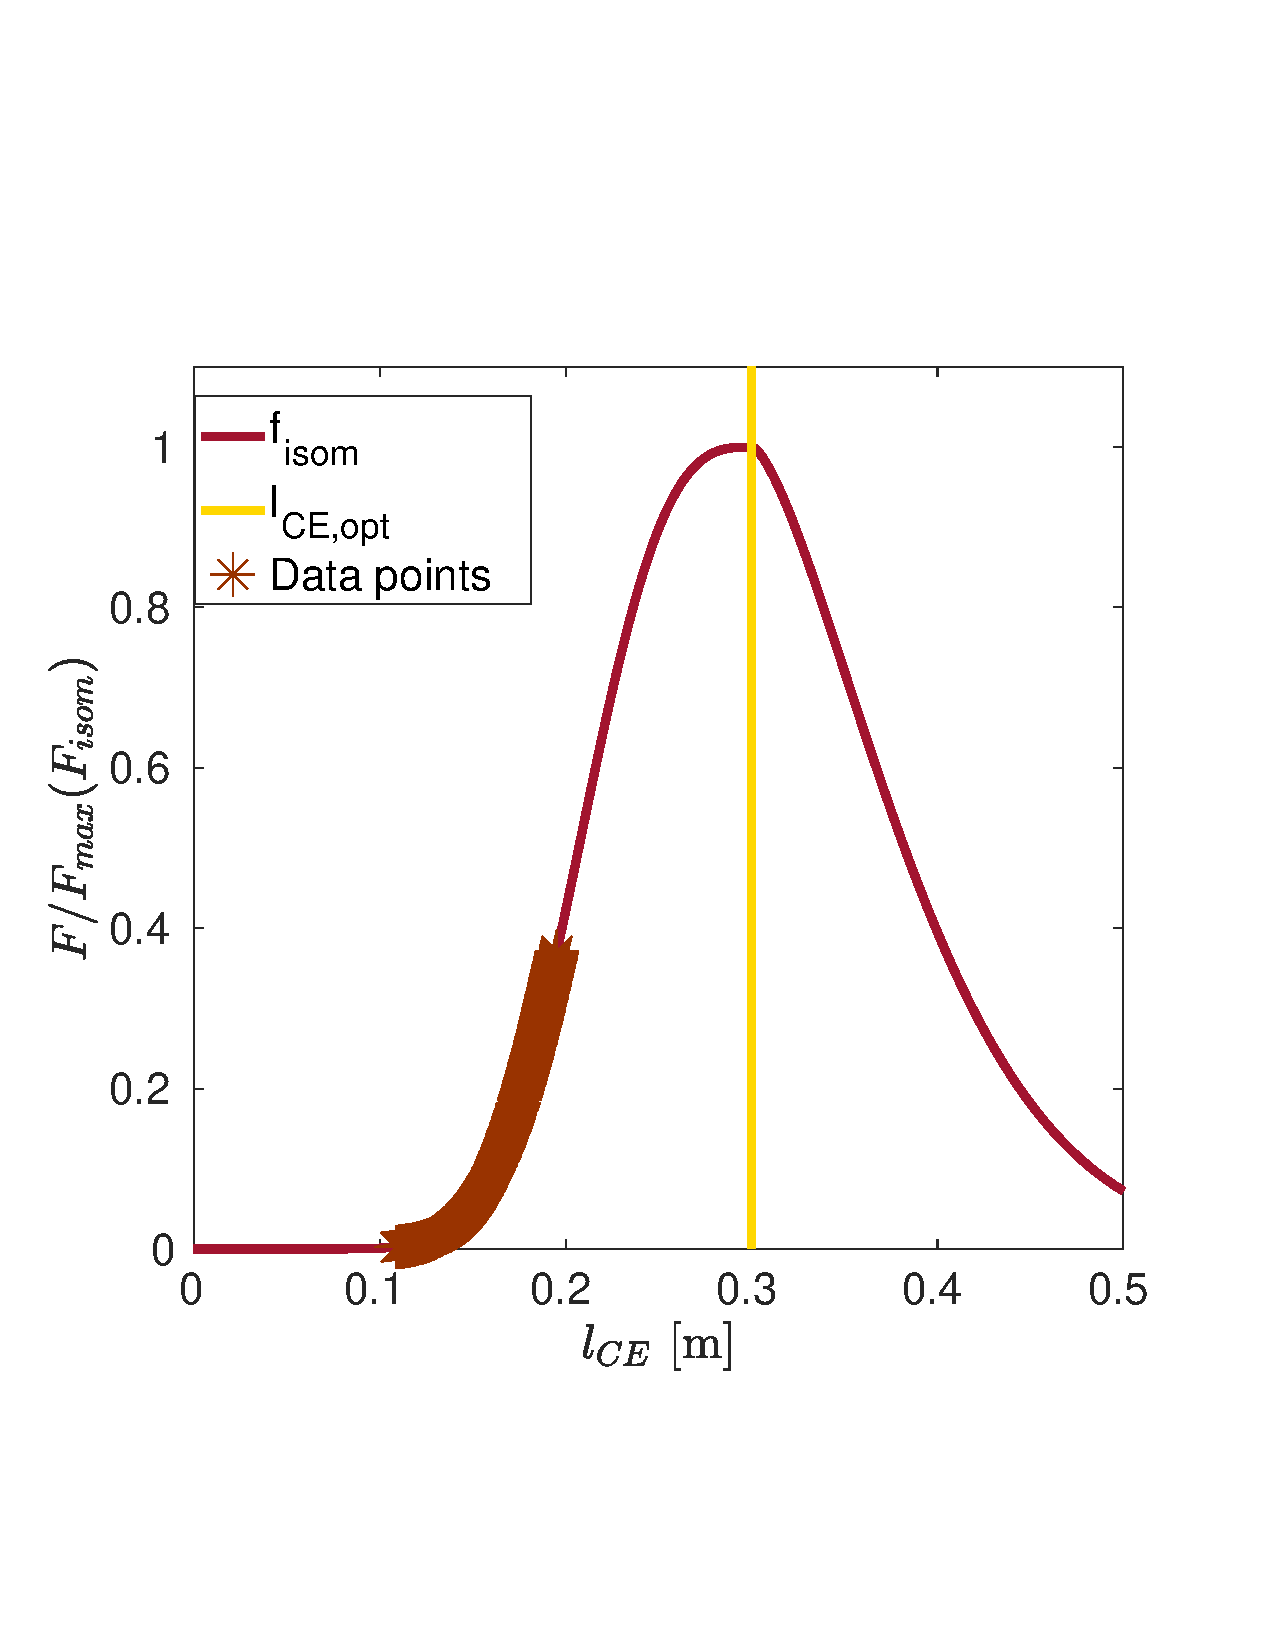
\includegraphics[width=\textwidth]{images/summer_school_study/biceps_initial.pdf}%
    \caption{Model with generic parametrization and training data points.}%
    \label{fig:biceps_a}%
  \end{subfigure}%
  \quad
  \begin{subfigure}[t]{0.47\textwidth}%
    \centering%
    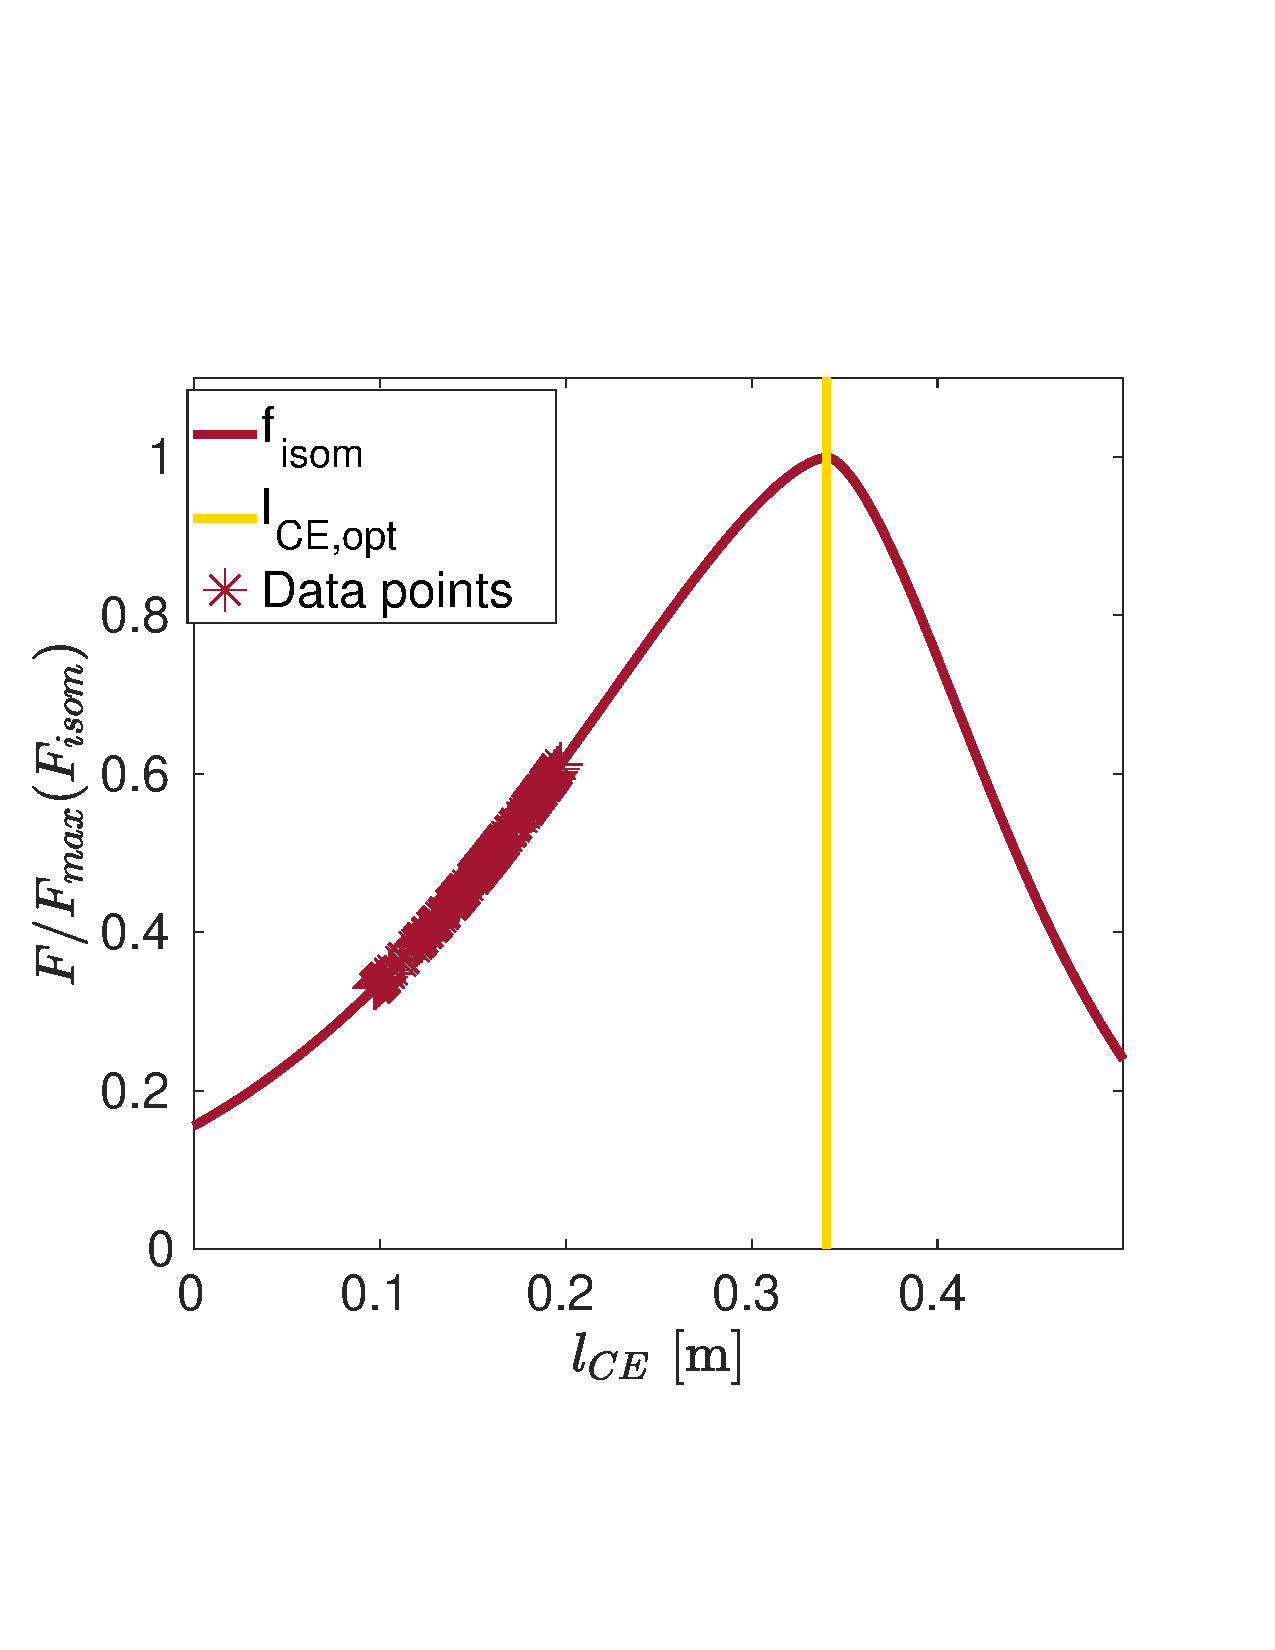
\includegraphics[width=\textwidth]{images/summer_school_study/biceps_optimized.pdf}%
    \caption{Model with subject-specific parametrization and training data points.}%
    \label{fig:biceps_b}%
  \end{subfigure}%
  \caption{Isometric force-length relation of the CE for the biceps model, analogous to \cref{fig:force_curves_generic_length}.}%
  \label{fig:biceps_working_area}%
\end{figure}%


\begin{figure}%
  \centering%
  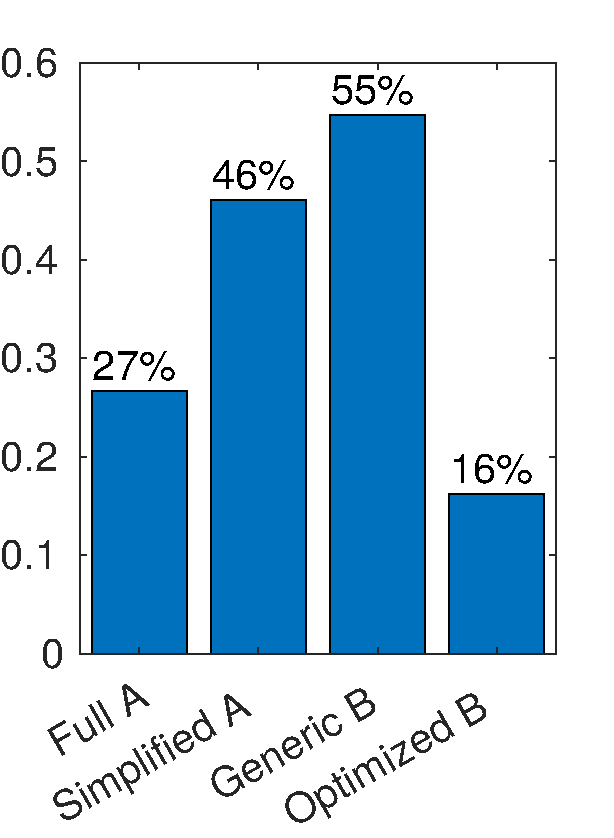
\includegraphics[width=0.35\textwidth]{images/summer_school_study/nrmse.pdf}%
  \caption{Normalized Root Mean Square errors (NRMSE) of the validation trials between the respective models and the measured values. A lower error value means a better fit.}%
  \label{fig:nrmse}%
\end{figure}%

\section{Conclusion}\label{sec:study_conclusion}
In this study, elbow torques during flexion and extension of the upper arm was predicted from motion capture information and EMG measurements. Two models, A and B, were developed. Model A is non-parametric and uses Gaussian Process Regression. Model B is biophysically informed and involves two Hill-type muscle models for biceps and triceps. Experiments were conducted to generate training data that was used for model parameter identification. The two models were evaluated using experimental validation data.

Regarding the implementation, model A requires low effort and no special knowledge about the model, except when motion data is preprocessed for a specific subject. Model B needs expert knowledge about the biophysical structure and the implementation of all comprised models.

Similar holds for the offline training phase. Here, an advantage of model A is that additional information, e.g. from neighbouring muscles or additional sensors can easily be added. Instead, Model B incorporates a-priori information about the functioning of the muscular system and allows to aid the parameter identification step by enforcing physiological constraints $\Theta$ for the parameters.

Considering the prediction error, both models were able to predict the level of torque reasonably. 
\Cref{fig:nrmse} showed the best score for model A, followed by model B. It was also shown that the generic parametrization of model B does not yield a useful prediction. The same is true for a simplified application of model A, where the elbow torque was used as training input instead of derived quantities from the motion capture system that required a complex preprocessing step.

Both models provide possiblities to assess the level of confidence of their predictions. With model A, confidence intervals can be computed directly from the Gaussian Processes. Their usefulness was shown in the validation where regions with large errors also had a large confidence interval. Model B allows insight into force-length and force-velocity characteristics of the two involved muscles. The operating range of the muscle during the experiments can be visualized and allows to assess whether the desired model features were covered by the training phase and, thus, promise a good prediction.

In our study, runtimes were low for model A and high for model B in both offline and online phases. However, this is due to our prototypical implementation of model B. For larger data sizes and more sophisticated implementation, the reverse effect is expected. The runtime complexity for the training phase is better for model B (linear in time) compared to model A (cubic in time). For the online phase, costly integration over data points is needed for model A whereas model B directly provides a differential equation of the system that can be solved efficiently. 

When targeted at real-time application, such as for powered orthoses and prostheses or exoskeletons, both models could be considered. Model A fits the use case of a device that could be (re-)calibrated by the patient itself. Because of the built-in confidence estimation, compliance and safety could be ensured more easily even for imperfect training.
Model B would need a controlled environment such as a specialist's laboratory and careful assistence for the calibration process.
After calibration it would promise a more natural and more responsive experience because of the subject-specific model and possibly smaller computation times.

This study reveiled some advantages of biophysically informed models for prediction of human movements. The kinematics and the individual muscle dynamics were modeled close to the understanding of the system in-vivo. However, several aspects where not modeled as detailed as possible. The pathway from neural stimulation to excitation and activation of the muscle, the recruitment strategies including different motor units, neural feedback loops as well as effects stemming from the 3D geometry of the muscle were not considered. A more detailed, biophysically informed model including these properties will be described in the following sections of the chapter.


  \chapter{Formulation of electrophysiology and muscle contraction}
    - electrophysiology introduction
    \section{State of the art}
    - Hodgkin-Huxley, shorten, advanced models, how it gets solved
    \section{discretization}
    - discretization of electrophysiology, operator splitting
    \section{Standard for formulation of models}
    - cellml introduction
    \section{Bidomain}
    - EMG
    \section{Multidomain}
    - multidomain formulation
    \section{Formulation of solid mechanics}
    - basics solid mechanics framework, material modeling, 
    
  \section{Simulation workflow}
  - simulation workflow of skeletal muscle
  
  \chapter{Numeric}
  \section{Fundamentals of the discretization}
    \section{Finite element method}
    - basics FEM formulation of Laplace operator and diffusion equation, boundary conditions
    \section{Incompressible nonlinear solid mechanics}
    - incompressibility, penalty formulation vs. mixed formulation\\
    - governing nonlinear eq.\\
    - jacobian
  \section{Numerical schemes}
    \section{time stepping schemes}
    \section{linear system solvers}
    \section{newton algorithm}
    
  \chapter{Simulation software}
    \section{General aspects}
    \section{Detail}
  % 
  \chapter{Simulation software}
    \section{State of the art}
    - review on bioengineering simulation frameworks 
    
    \section{OpenCMISS}
  - OpenCMISS introduction, iron zinc cmgui, unstructured\\
  
  - Strang splitting, solvers 1D\\
  - improved interpolation\\
  - parallelization, issue with 1D \\
  - 3D parallelization strategies\\
  - design flaws, memory\\
    % untergliedern, z.B. schnittstellen parall etc.
    \section{The simulation framework \emph{opendihu}}
    - modularity of opendihu, concepts (python c++ build system)
    \section{Overview of discretization features}
    - feature overview, implemented equations, ansatz functions, meshes
    \section{Input and output}
    - file i/o parallel, i: only local data important for high parallelism, o: paraview
    \section{In-situ visualization}
    - in-situ
    \section{Details on the implementation}
    \section{Representation of structured meshes}
    \section{Parallel data handling}
    - data structures, petsc variables, partitioning, ghost communication
    \section{Implementation of boundary conditions}
    - Neumann, Dirichlet boundary conditions
    \section{Implementation of material formulation and automatic derivation of derivatives}
    - implementation of solid mechanics with analytic differentiation
    
    \section{efficient and configurable data transfer}
    - data layout details, efficient transfer of variables between solvers
    \section{Mapping between meshes}
    - parallel mapping between meshes, invertability of index space represesantion
    \section{An efficient solver to the Monodomain equation}    
    - cellml code generator and its optimizations - openmp, simd, vc
    \section{Details on the partitioning}
    - fibers emg structure and partitioning
    \section{Parallelization of the multidomain system}
    - multidomain parallelization, reordering of matrix
    \section{load balancing}
    - load balancing on fiber level
  \chapter{External coupling}
    - introduction to external coupling, precice
    \section{coupling with FEBio}
    \section{coupling with AceFEM}
  
  \chapter{An algorithm for mesh generation}
    - introduction, need for fiber and 3d mesh
    \section{State of the art}
    - literature, laplace potential flow idea
    \section{Data preprocessing}
    - visual human dataset, methods to extract surface, approximation by spline surfaces
    \section{Outline of the algorithm}
    - pseudo code
    \section{Plane mesh smoothing}
    \section{Parallelization}
    \section{Generation of fiber meshes}
    - generation of muscle mesh, 3D and fibers, also in parallel
  
  \chapter{Simulation scenarios}
    \section{Simulation of electromyography with fiber-based formulation}
      - scenario static-biceps-emg, composite meshes
    \section{Simulation of electromyography with multidomain formulation}
    \section{Muscle contraction with fiber-based formulation}
      - fibers with contraction
    \section{Muscle contraction with multidomain formulation}
  \chapter{Technical simulation results}
    \section{Runtime evaluation}
    - results and experiments, runtime, peak performance\\
    - monodomain runtime comparison OpenCMISS opendihu
    \section{parallel partitioning}
    - parallel partitioning and weak scaling, opencmiss and opendihu 
    \section{memory consumption}
    - memory scaling OpenCMISS
  \chapter{biomechanical simulation results}
    \section{Simulation of fatigue}
    - monodomain, hh  shorten, fatigue effects
    \section{Simulation of EMG}
    - static biceps emg\\
    - fibers with contraction\\
    - multidomain with fat layer\\
    - multidomain with contraction\\

\part{Soft tissue robotics}
\chapter{...}
  - introduction, handling flexible objects, overview of different object types\\
  - basics Lagrange formulation of cable\\
  - cable with friction on surface\\
  - placing cable\\
  - peg-in-hole, with sparse grids\\
  - simulation of 2d tissue\\
  - gripping point estimation\\
  
  \cite{Maier2021}
  
\part{Conclusion}

% -------------- Literaturseite --------------------
\newpage
%\bibliography{references}{}
%\bibliographystyle{abbrv}
\printbibliography[%
  % change title
  title=Bibliography
]


% -------------- Anhang ------------
%\appendix
%\input{8_anhang.tex}

\end{document}

%\input{preambule/footer}
